% =============================================================================
% PyCore microarchitecture diagram atlas
% =============================================================================
% Build from this directory:
%   pdflatex pycore_diagrams.tex && pdflatex pycore_diagrams.tex
% Requires: article, tikz, booktabs, hyperref, geometry, microtype, amsmath
% Figure sources: figures/fig_*.tex   styles: figures/tikz_styles.tex
% =============================================================================
\documentclass[11pt,a4paper]{article}

\usepackage[margin=0.85in]{geometry}
\usepackage{microtype}
\usepackage[T1]{fontenc}
\usepackage{lmodern}
\usepackage{booktabs}
\usepackage{amsmath}
\usepackage{amssymb}
\usepackage{xcolor}
\usepackage{caption}
\usepackage{hyperref}
\usepackage{tikz}
\usetikzlibrary{arrows.meta,positioning,fit,calc,backgrounds,decorations.pathreplacing}

% Shared TikZ style for the PyCore diagram atlas.
% Input from the article preamble. A standalone figure can use the same file.
\definecolor{pyedge}{RGB}{55,65,75}
\definecolor{pyctl}{RGB}{214,228,240}
\definecolor{pymem}{RGB}{210,230,214}
\definecolor{pyrf}{RGB}{255,236,186}
\definecolor{pyacc}{RGB}{226,214,240}
\definecolor{pyex}{RGB}{255,214,180}
\definecolor{pytrap}{RGB}{245,208,208}
\definecolor{pyres}{RGB}{236,236,236}
\definecolor{pyink}{RGB}{232,220,228}
\definecolor{pyhi}{RGB}{255,248,220}

\tikzset{
  pybox/.style={
    draw=pyedge, line width=0.55pt, rounded corners=1.5pt,
    align=center, inner sep=3.2pt, font=\scriptsize\sffamily,
    minimum height=7.2mm
  },
  ctl/.style={pybox, fill=pyctl},
  mem/.style={pybox, fill=pymem},
  rf/.style={pybox, fill=pyrf},
  acc/.style={pybox, fill=pyacc},
  ex/.style={pybox, fill=pyex},
  trap/.style={pybox, fill=pytrap},
  res/.style={pybox, fill=pyres, dashed},
  ink/.style={pybox, fill=pyink},
  hi/.style={pybox, fill=pyhi},
  arr/.style={-{Latex[length=1.7mm,width=1.35mm]}, draw=pyedge, line width=0.65pt},
  darr/.style={arr, dashed},
  bus/.style={
    draw=pyedge, fill=black!4, font=\tiny\ttfamily,
    inner sep=2.2pt, align=center, rounded corners=1pt
  },
  slot/.style={
    draw=pyedge, line width=0.45pt, align=center,
    font=\tiny\sffamily, inner sep=2pt, minimum height=5.6mm
  },
  grp/.style={
    draw=pyedge, dashed, rounded corners=2.5pt, inner sep=5pt, line width=0.5pt
  },
  anno/.style={font=\tiny\sffamily, text=black!75, align=center},
  every picture/.append style={font=\scriptsize\sffamily, line join=round}
}


\hypersetup{
  colorlinks=true,
  linkcolor=black,
  urlcolor=blue!50!black,
  citecolor=black
}

\captionsetup{font=small,labelfont=bf,skip=6pt}

\title{PyCore Microarchitecture Diagrams\\
\large A figure atlas for the research paper}
\author{PyCore systems notes\\
\texttt{docs/paper/systems/pycore\_diagrams.tex}}
\date{October 2026}

\begin{document}
\maketitle

\begin{abstract}
PyCore is a research CPU whose instruction set is a CPython~3.14 bytecode subset.
This note is a diagram atlas of the hart as built: the two-core system, the control
states, the tagged register ring, the memory hierarchy, and every accelerator
(integer, floating-point, string, and the collector), plus the container layouts
those accelerators read.
Each figure is drawn against the RTL names in \texttt{pycore/rtl} so it can be
lifted into a paper with the caption edited and the geometry left alone.
Numbers are the parameters in \texttt{pycore\_defs.svh}.
The call binder's internal phases stay in the sibling note \texttt{call\_fsm.tex}.
\end{abstract}

\tableofcontents
\listoffigures
\newpage

\section{How to use these figures}
\label{sec:how}

The atlas is the block diagram a reader needs before any opcode table.
It is not a second architecture manual: \texttt{pycore/docs/architecture.md}
remains the prose source of truth, and a figure that disagrees with that file
or with the RTL is wrong.

\paragraph{Color.}
Blue is control state.
Green is memory.
Amber is the register file.
Purple is an accelerator.
Orange is excore or the mailbox.
Red is a trap.
A dashed box is specified and not built, or reserved.

\paragraph{Lifting a figure.}
Each figure is a separate file under \texttt{figures/}, and every picture
uses the styles in \texttt{tikz\_styles.tex}.
Copy one \texttt{tikzpicture} into the paper, input the style file from the
preamble, and rewrite the caption for the venue.
The labels are RTL identifiers on purpose (\texttt{rf\_wm\_r},
\texttt{S\_STRACC}, \texttt{CP\_DICT\_PROBE}).

\paragraph{What is in scope.}
The hart, its memory system, the accelerators, the container object model,
and the excore contract.
Out of scope are the on-device compiler, the firmware bodies under
\texttt{pycore\_firmware/}, and the excore pipeline itself.
Those have their own documents.

\paragraph{Three facts that keep the diagrams honest.}
The core is multi-cycle and non-pipelined: one instruction is in flight.
Integers are a signed 64-bit fast path; overflow traps instead of growing a
big integer.
The collector is built and off unless the simulation is started with
\texttt{+GC\_EN=1}.

\section{The machine}
\label{sec:machine}

% Two-core system and the pycore hart. Requires tikz_styles.tex.
\begin{figure}[p]
\centering
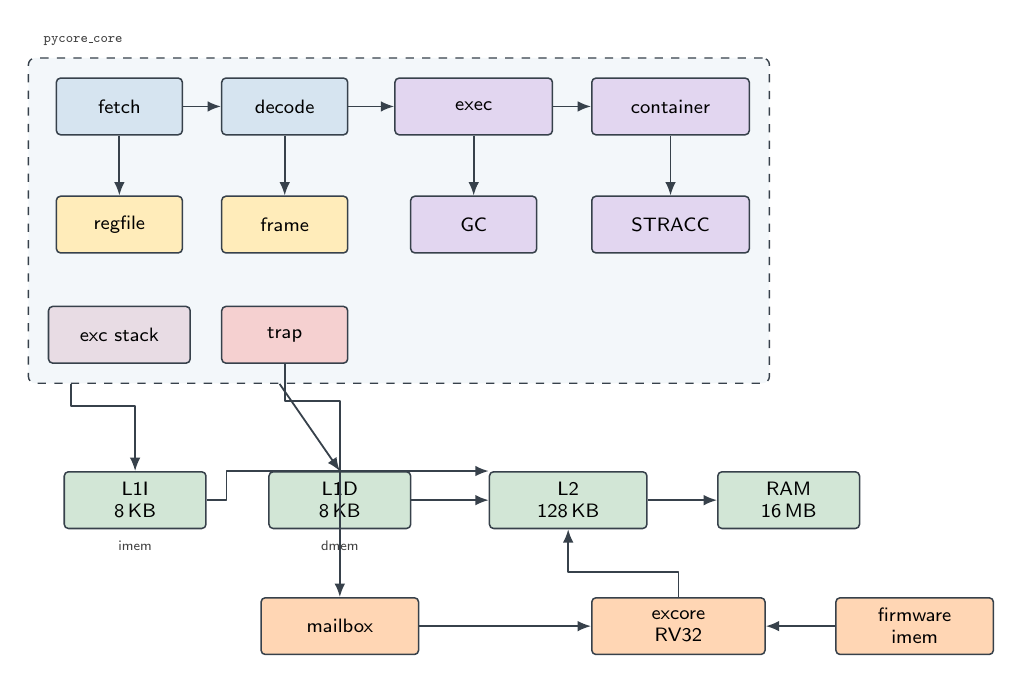
\begin{tikzpicture}[x=1cm,y=1cm]
  \node[ctl, minimum width=16mm] (fetch) at (1.5,7.35) {fetch};
  \node[ctl, minimum width=16mm] (dec) at (3.6,7.35) {decode};
  \node[acc, minimum width=20mm] (exec) at (6.0,7.35) {exec};
  \node[acc, minimum width=20mm] (cont) at (8.5,7.35) {container};
  \node[rf, minimum width=16mm] (rf) at (1.5,5.85) {regfile};
  \node[rf, minimum width=16mm] (frm) at (3.6,5.85) {frame};
  \node[acc, minimum width=16mm] (gc) at (6.0,5.85) {GC};
  \node[acc, minimum width=20mm] (str) at (8.5,5.85) {STRACC};
  \node[ink, minimum width=18mm] (exc) at (1.5,4.45) {exc stack};
  \node[trap, minimum width=16mm] (trap) at (3.6,4.45) {trap};

  \begin{scope}[on background layer]
    \node[grp, fill=pyctl!30, inner sep=7pt,
          fit=(fetch)(cont)(exc)(str)] (core) {};
  \end{scope}
  \node[anno, anchor=south west, font=\tiny\ttfamily]
    at ($(core.north west)+(0.08,0.02)$) {pycore\_core};

  \node[mem, minimum width=18mm] (l1i) at (1.7,2.35) {L1I\\8\,KB};
  \node[mem, minimum width=18mm] (l1d) at (4.3,2.35) {L1D\\8\,KB};
  \node[mem, minimum width=20mm] (l2) at (7.2,2.35) {L2\\128\,KB};
  \node[mem, minimum width=18mm] (ram) at (10.0,2.35) {RAM\\16\,MB};

  \node[ex, minimum width=20mm] (mb) at (4.3,0.75) {mailbox};
  \node[ex, minimum width=22mm] (excore) at (8.6,0.75) {excore\\RV32};
  \node[ex, minimum width=20mm] (fw) at (11.6,0.75) {firmware\\imem};

  \draw[arr] (fetch) -- (dec);
  \draw[arr] (dec) -- (exec);
  \draw[arr] (exec) -- (cont);
  \draw[arr] (fetch) -- (rf);
  \draw[arr] (dec) -- (frm);
  \draw[arr] (exec) -- (gc);
  \draw[arr] (cont) -- (str);

  \draw[arr] ($(core.south west)+(0.55,0)$) -- ++(0,-0.28) -| (l1i.north);
  \draw[arr] ($(core.south west)+(3.2,0)$) -- (l1d.north);
  \draw[arr] (l1i.east) -- ++(0.25,0) |- (l2.north west);
  \draw[arr] (l1d.east) -- (l2.west);
  \draw[arr] (l2.east) -- (ram.west);
  \draw[arr] (excore.north) -- ++(0,0.32) -| (l2.south);
  \draw[arr] (fw.west) -- (excore.east);
  \draw[arr] (trap.south) -- ($(trap.south |- core.south)+(0,-0.22)$) -| (mb.north);
  \draw[arr] (mb.east) -- (excore.west);

  \node[anno, anchor=north] at ($(l1i.south)+(0,-0.02)$) {imem};
  \node[anno, anchor=north] at ($(l1d.south)+(0,-0.02)$) {dmem};
\end{tikzpicture}
\caption{Two-core system.
PyCore is the CPython-bytecode hart.
Excore is an RV32 multicycle hart that finishes recoverable traps in firmware.
Instruction memories stay private: fetch uses L1I, and excore has its own firmware memory.
The shared resource is the data heap.
PyCore's data masters share one port into L1D.
Excore's slot port attaches at L2 and never at L1D.
PyCore is frozen in \texttt{S\_TRAP\_MARSHAL} / \texttt{S\_TRAP\_WAIT} while excore owns memory.
\texttt{pycore\_system} is the same hart with the mailbox tied off.}
\label{fig:twocore}
\end{figure}

\begin{figure}[p]
\centering
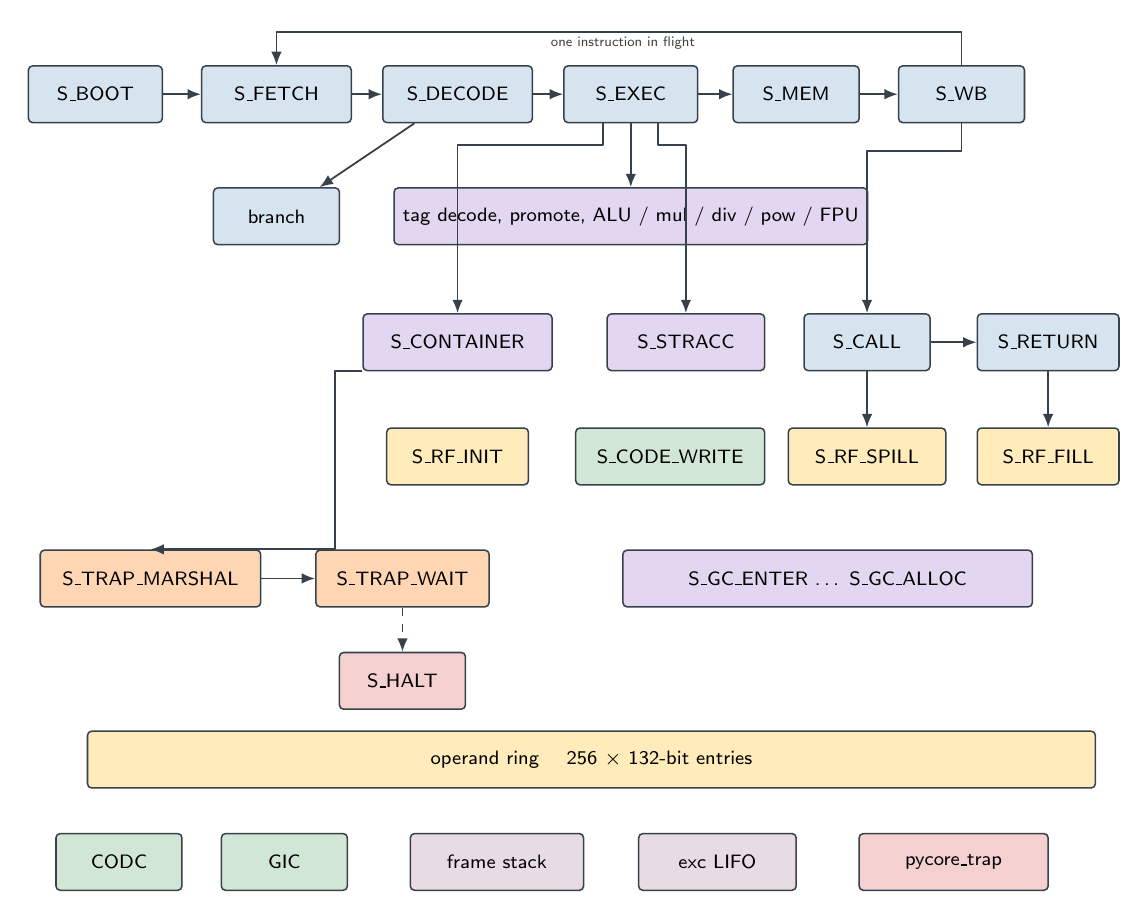
\begin{tikzpicture}[x=1cm,y=1cm]
  \node[ctl, minimum width=17mm] (boot) at (0.9,8.6) {S\_BOOT};
  \node[ctl, minimum width=19mm] (fe) at (3.2,8.6) {S\_FETCH};
  \node[ctl, minimum width=19mm] (id) at (5.5,8.6) {S\_DECODE};
  \node[ctl, minimum width=17mm] (ex) at (7.7,8.6) {S\_EXEC};
  \node[ctl, minimum width=16mm] (mem) at (9.8,8.6) {S\_MEM};
  \node[ctl, minimum width=16mm] (wb) at (11.9,8.6) {S\_WB};

  \node[acc, minimum width=46mm] (fabric) at (7.7,7.05)
    {tag decode, promote, ALU / mul / div / pow / FPU};
  \node[ctl, minimum width=16mm] (br) at (3.2,7.05) {branch};

  \node[acc, minimum width=24mm] (cont) at (5.5,5.45) {S\_CONTAINER};
  \node[acc, minimum width=20mm] (sa) at (8.4,5.45) {S\_STRACC};
  \node[ctl, minimum width=16mm] (call) at (10.7,5.45) {S\_CALL};
  \node[ctl, minimum width=18mm] (ret) at (13.0,5.45) {S\_RETURN};

  \node[rf, minimum width=18mm] (init) at (5.5,4.0) {S\_RF\_INIT};
  \node[mem, minimum width=24mm] (cw) at (8.2,4.0) {S\_CODE\_WRITE};
  \node[rf, minimum width=20mm] (spill) at (10.7,4.0) {S\_RF\_SPILL};
  \node[rf, minimum width=18mm] (fill) at (13.0,4.0) {S\_RF\_FILL};

  \node[ex, minimum width=28mm] (mar) at (1.6,2.45) {S\_TRAP\_MARSHAL};
  \node[ex, minimum width=22mm] (wait) at (4.8,2.45) {S\_TRAP\_WAIT};
  \node[trap, minimum width=16mm] (halt) at (4.8,1.15) {S\_HALT};
  \node[acc, minimum width=52mm] (gc) at (10.2,2.45) {S\_GC\_ENTER \ldots\ S\_GC\_ALLOC};

  \node[rf, minimum width=128mm] (ring) at (7.2,0.15)
    {operand ring \quad 256 $\times$ 132-bit entries};

  \node[mem, minimum width=16mm] (codc) at (1.2,-1.15) {CODC};
  \node[mem, minimum width=16mm] (gic) at (3.3,-1.15) {GIC};
  \node[ink, minimum width=22mm] (frame) at (6.0,-1.15) {frame stack};
  \node[ink, minimum width=20mm] (excst) at (8.8,-1.15) {exc LIFO};
  \node[trap, minimum width=24mm] (tblock) at (11.8,-1.15) {pycore\_trap};

  \draw[arr] (boot) -- (fe);
  \draw[arr] (fe) -- (id);
  \draw[arr] (id) -- (ex);
  \draw[arr] (ex) -- (mem);
  \draw[arr] (mem) -- (wb);
  \draw[arr] (wb.north) -- ++(0,0.42) -| (fe.north);
  \draw[arr] (ex) -- (fabric);
  \draw[arr] (id) -- (br);
  \draw[arr] (ex.south) ++(-0.35,0) -- ++(0,-0.28) -| (cont.north);
  \draw[arr] (ex.south) ++(0.35,0) -- ++(0,-0.28) -| (sa.north);
  \draw[arr] (wb.south) -- ++(0,-0.35) -| (call.north);
  \draw[arr] (call) -- (ret);
  \draw[arr] (call) -- (spill);
  \draw[arr] (ret) -- (fill);
  \draw[arr] (cont.south west) -- ++(-0.35,0) |- (mar.north);
  \draw[arr] (mar) -- (wait);
  \draw[darr] (wait) -- (halt);

  \node[anno] at (7.6,9.25) {one instruction in flight};
\end{tikzpicture}
\caption{PyCore hart.
The machine is multi-cycle: one instruction is in flight, so the register file needs no forwarding.
The steady path is fetch, decode, execute, a thin memory stage, and writeback.
Container operations, the string accelerator, and calls leave that path and retire from their own states.
\texttt{S\_MEM} serves the internal pointer opcodes.
Image bytecode reaches the heap from the container FSM, calls, STRACC, and the collector.
CODC and GIC are combinational result caches, not line caches.
State transitions are Figure~\ref{fig:fsm}.}
\label{fig:hart}
\end{figure}


PyCore's ISA is the bytecode, not a RISC that a compiler lowers bytecode onto.
That is why containers, calls, and strings are states in the same control
machine as fetch, rather than coprocessor instructions issued by a host core.

Table~\ref{tab:states} is the state register in \texttt{pycore\_core.sv}.
Figure~\ref{fig:fsm} draws the edges that matter for a paper; it omits the
self-loops where a state waits on \texttt{ack} or \texttt{stall\_o}.

\begin{table}[htbp]
\centering
\caption{Control states.}
\label{tab:states}
\footnotesize
\begin{tabular}{@{}clp{0.55\textwidth}@{}}
\toprule
Id & State & Role \\
\midrule
0 & \texttt{S\_FETCH} & Present one real instruction. \\
1 & \texttt{S\_DECODE} & Form ring addresses and latch operands. \\
2 & \texttt{S\_EXEC} & Execute fabric and branch unit. \\
3 & \texttt{S\_MEM} & Pointer load/store only. \\
4 & \texttt{S\_WB} & One register write, stack-pointer update. \\
5 & \texttt{S\_HALT} & Fatal trap. Architectural state freezes. \\
6 & \texttt{S\_CALL} & Bind arguments and push a frame. \\
7 & \texttt{S\_RETURN} & Pop a frame and write the result. \\
8 & \texttt{S\_CONTAINER} & Heap and name operations. \\
9 & \texttt{S\_BOOT} & Read the boot record. \\
10 & \texttt{S\_TRAP\_MARSHAL} & Hand operands to the mailbox. \\
11 & \texttt{S\_TRAP\_WAIT} & Apply \texttt{COMPLETED} / \texttt{RETRY} / \texttt{FATAL}. \\
12 & \texttt{S\_STRACC} & String accelerator owns the data port. \\
13 & \texttt{S\_RF\_SPILL} & Evict a ring prefix to the spill LIFO. \\
14 & \texttt{S\_RF\_FILL} & Restore a spilled prefix. \\
15 & \texttt{S\_RF\_INIT} & Clear unfilled locals to \texttt{UNINIT}, 32 at a time. \\
16 & \texttt{S\_CODE\_WRITE} & Core writes code RAM (blit / patch). \\
17 & \texttt{S\_GC\_ENTER} & Drain an outstanding data beat, start the engine. \\
18 & \texttt{S\_GC\_ROOTS} & Stream register and ring roots. \\
19 & \texttt{S\_GC\_RUN} & Mark and sweep. \\
20 & \texttt{S\_GC\_ALLOC} & Grant a free run, or collect if the list is empty. \\
\bottomrule
\end{tabular}
\end{table}

% Core control FSM. Requires tikz_styles.tex.
\begin{figure}[p]
\centering
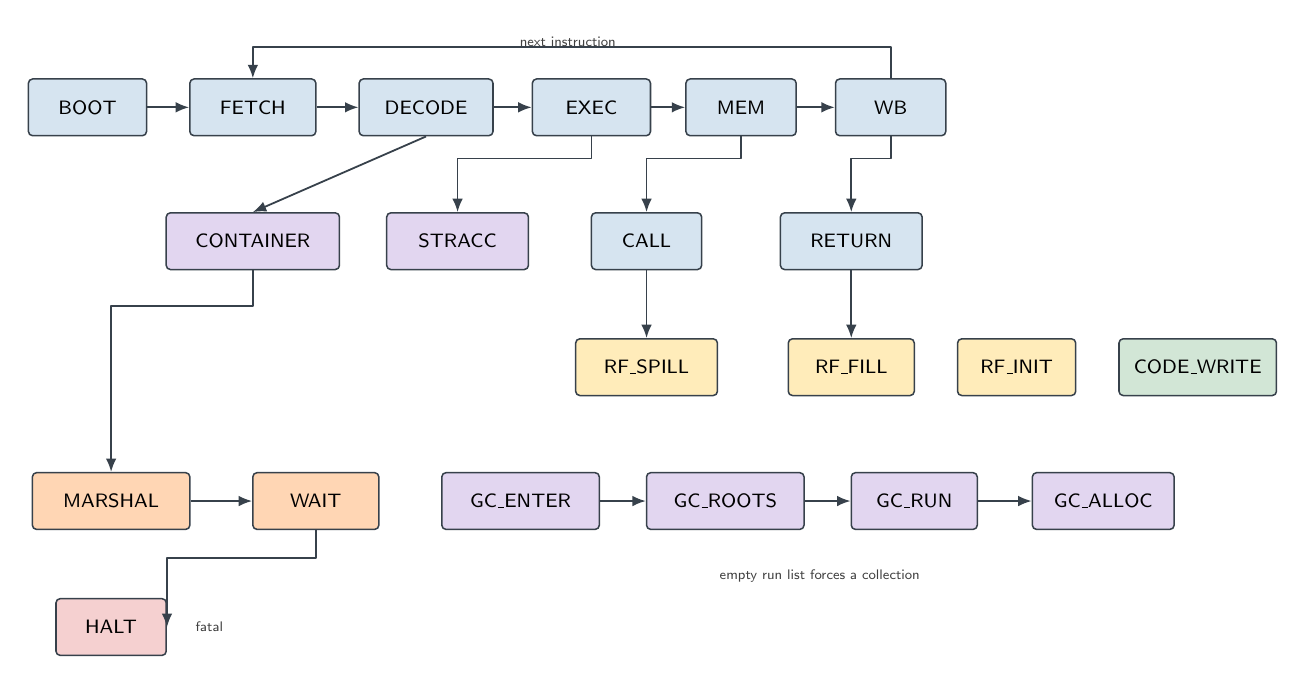
\begin{tikzpicture}[x=1cm,y=1cm]
  % Main pipeline
  \node[ctl, minimum width=15mm] (boot) at (0.9,7.6) {BOOT};
  \node[ctl, minimum width=16mm] (fetch) at (3.0,7.6) {FETCH};
  \node[ctl, minimum width=17mm] (dec) at (5.2,7.6) {DECODE};
  \node[ctl, minimum width=15mm] (exec) at (7.3,7.6) {EXEC};
  \node[ctl, minimum width=14mm] (mems) at (9.2,7.6) {MEM};
  \node[ctl, minimum width=14mm] (wb) at (11.1,7.6) {WB};

  % Departures from EXEC / WB
  \node[acc, minimum width=22mm] (cont) at (3.0,5.9) {CONTAINER};
  \node[acc, minimum width=18mm] (sa) at (5.6,5.9) {STRACC};
  \node[ctl, minimum width=14mm] (call) at (8.0,5.9) {CALL};
  \node[ctl, minimum width=18mm] (ret) at (10.6,5.9) {RETURN};

  \node[rf, minimum width=18mm] (spill) at (8.0,4.3) {RF\_SPILL};
  \node[rf, minimum width=16mm] (fill) at (10.6,4.3) {RF\_FILL};
  \node[rf, minimum width=15mm] (init) at (12.7,4.3) {RF\_INIT};
  \node[mem, minimum width=20mm] (cw) at (15.0,4.3) {CODE\_WRITE};

  % Trap and GC, kept on their own rows
  \node[ex, minimum width=20mm] (mar) at (1.2,2.6) {MARSHAL};
  \node[ex, minimum width=16mm] (wait) at (3.8,2.6) {WAIT};
  \node[trap, minimum width=14mm] (halt) at (1.2,1.0) {HALT};

  \node[acc, minimum width=20mm] (ent) at (6.4,2.6) {GC\_ENTER};
  \node[acc, minimum width=20mm] (roots) at (9.0,2.6) {GC\_ROOTS};
  \node[acc, minimum width=16mm] (run) at (11.4,2.6) {GC\_RUN};
  \node[acc, minimum width=18mm] (alloc) at (13.8,2.6) {GC\_ALLOC};

  \draw[arr] (boot) -- (fetch);
  \draw[arr] (fetch) -- (dec);
  \draw[arr] (dec) -- (exec);
  \draw[arr] (exec) -- (mems);
  \draw[arr] (mems) -- (wb);
  \draw[arr] (wb.north) -- ++(0,0.4) -| (fetch.north);

  \draw[arr] (exec.south) -- ++(0,-0.28) -| (sa.north);
  \draw[arr] (dec.south) -- (cont.north);
  \draw[arr] (wb.south) -- ++(0,-0.28) -| (ret.north);
  \draw[arr] (mems.south) -- ++(0,-0.28) -| (call.north);

  \draw[arr] (call) -- (spill);
  \draw[arr] (ret) -- (fill);

  \draw[arr] (cont.south) -- ++(0,-0.45) -| (mar.north);
  \draw[arr] (mar) -- (wait);
  \draw[arr] (wait.south) -- ++(0,-0.35) -| (halt.east);
  \draw[arr] (ent) -- (roots);
  \draw[arr] (roots) -- (run);
  \draw[arr] (run) -- (alloc);

  \node[anno, anchor=south] at (7.0,8.25) {next instruction};
  \node[anno, anchor=west] at (2.15,1.0) {fatal};
  \node[anno, anchor=north] at (10.2,1.85) {empty run list forces a collection};
\end{tikzpicture}
\caption{Control states in \texttt{pycore\_core}.
The top row is the steady path; the arrow above it is the return to fetch.
Solid edges are completions, not the self-loops that wait on \texttt{ack} or \texttt{stall\_o}.
Any latched fatal trap forces \texttt{S\_HALT}.
\texttt{S\_FETCH} holds until \texttt{pycore\_fetch} presents a real instruction
(\texttt{CACHE} skipped, \texttt{EXTENDED\_ARG} folded inside the fetch unit).
Recoverable traps leave the container FSM for \texttt{S\_TRAP\_MARSHAL} when \texttt{EXCORE\_EN=1}.
A collection that starts because an allocation does not fit enters \texttt{S\_GC\_ALLOC} directly.
An empty free-run list continues into \texttt{S\_GC\_ENTER}.}
\label{fig:fsm}
\end{figure}

\begin{figure}[htbp]
\centering
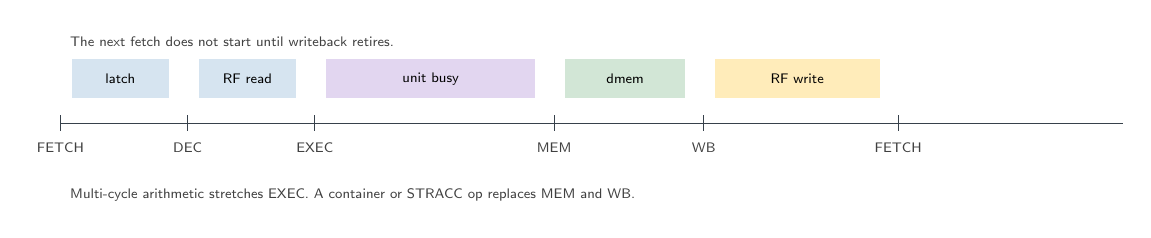
\begin{tikzpicture}[x=0.95cm,y=0.72cm]
  \draw[pyedge] (0,0) -- (14.2,0);
  \foreach \x/\lab in {0/FETCH, 1.7/DEC, 3.4/EXEC, 6.6/MEM, 8.6/WB, 11.2/FETCH} {
    \draw[pyedge] (\x,-0.12) -- (\x,0.16);
    \node[anno, anchor=north] at (\x,-0.16) {\lab};
  }
  \fill[pyctl] (0.15,0.45) rectangle (1.45,1.15);
  \fill[pyctl] (1.85,0.45) rectangle (3.15,1.15);
  \fill[pyacc] (3.55,0.45) rectangle (6.35,1.15);
  \fill[pymem] (6.75,0.45) rectangle (8.35,1.15);
  \fill[pyrf] (8.75,0.45) rectangle (10.95,1.15);
  \node[font=\tiny\sffamily] at (0.8,0.8) {latch};
  \node[font=\tiny\sffamily] at (2.5,0.8) {RF read};
  \node[font=\tiny\sffamily] at (4.95,0.8) {unit busy};
  \node[font=\tiny\sffamily] at (7.55,0.8) {dmem};
  \node[font=\tiny\sffamily] at (9.85,0.8) {RF write};
  \node[anno, anchor=west] at (0,1.45)
    {The next fetch does not start until writeback retires.};
  \node[anno, anchor=west] at (0,-1.25)
    {Multi-cycle arithmetic stretches EXEC. A container or STRACC op replaces MEM and WB.};
\end{tikzpicture}
\caption{One instruction in flight.
There is no EX/MEM or MEM/WB forwarding, no load-use interlock, and no branch flush of younger instructions.
Taken branches redirect \texttt{pycore\_fetch} on the next entry to \texttt{S\_FETCH}.
Decode reads \texttt{tos\_r} combinationally, so the address it forms already includes the previous instruction's stack update.}
\label{fig:inflight}
\end{figure}


\section{Tagged values}
\label{sec:tags}

Every architectural value is one 132-bit entry.
The tag is stored beside the payload so that a later custom register-file
macro can replace \texttt{pycore\_regfile} without a tag-lookup pipeline.

% Tagged value format. Requires tikz_styles.tex.
\begin{figure}[htbp]
\centering
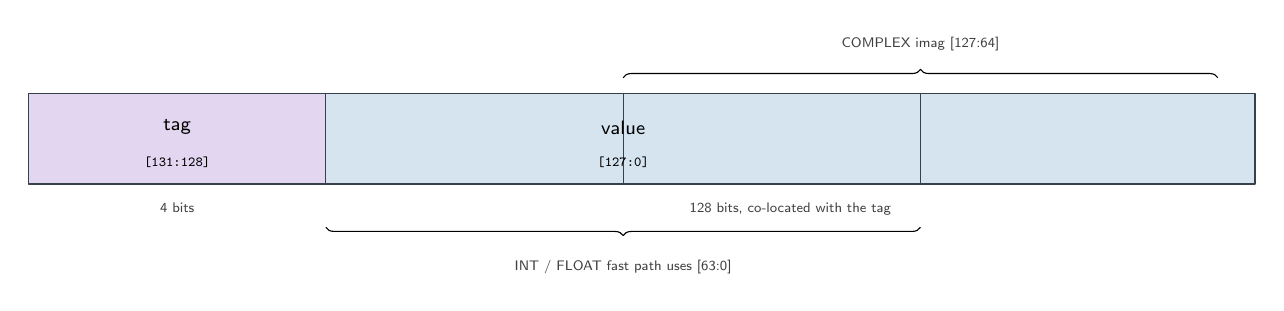
\begin{tikzpicture}[x=0.118cm,y=1cm]
  % 132 bits, drawn as tag + four 32-bit lanes of the value.
  \fill[pyacc] (0,0) rectangle (32,1.15);
  \fill[pyctl] (32,0) rectangle (132,1.15);
  \draw[pyedge, line width=0.6pt] (0,0) rectangle (132,1.15);
  \foreach \b in {32,64,96} {
    \draw[pyedge] (\b,0) -- (\b,1.15);
  }
  \node at (16,0.72) {\scriptsize tag};
  \node at (16,0.28) {\tiny\ttfamily [131:128]};
  \node at (64,0.72) {\scriptsize value};
  \node at (64,0.28) {\tiny\ttfamily [127:0]};
  \node[anno, anchor=north] at (16,-0.12) {4 bits};
  \node[anno, anchor=north] at (82,-0.12) {128 bits, co-located with the tag};
  \draw[decorate, decoration={brace, amplitude=3pt, mirror}]
    (32,-0.55) -- (96,-0.55);
  \node[anno] at (64,-1.05) {INT / FLOAT fast path uses [63:0]};
  \draw[decorate, decoration={brace, amplitude=3pt}]
    (64,1.35) -- (128,1.35);
  \node[anno] at (96,1.78) {COMPLEX imag [127:64]};
\end{tikzpicture}
\caption{Architectural register entry.
Every value the machine stores in the register file is 132 bits,
\texttt{\{tag[3:0], value[127:0]\}} (\texttt{PYCORE\_ENTRY\_WIDTH}).
The tag travels with the value, so a silicon register file does not need a second tag SRAM.
Helpers \texttt{pycore\_get\_tag}, \texttt{pycore\_get\_val}, and \texttt{pycore\_make\_entry} are the only legal way to slice an entry.}
\label{fig:entry}
\end{figure}

\begin{figure}[p]
\centering
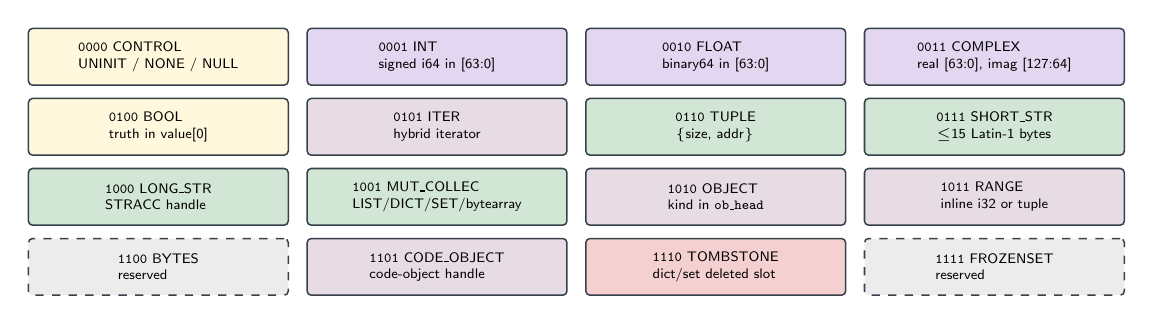
\begin{tikzpicture}[node distance=1.5mm and 2.2mm]
  \node[hi, minimum width=33mm, align=left, font=\tiny\sffamily] (t0)
    {\texttt{0000} CONTROL\\UNINIT / NONE / NULL};
  \node[acc, minimum width=33mm, align=left, font=\tiny\sffamily, right=of t0] (t1)
    {\texttt{0001} INT\\signed i64 in [63:0]};
  \node[acc, minimum width=33mm, align=left, font=\tiny\sffamily, right=of t1] (t2)
    {\texttt{0010} FLOAT\\binary64 in [63:0]};
  \node[acc, minimum width=33mm, align=left, font=\tiny\sffamily, right=of t2] (t3)
    {\texttt{0011} COMPLEX\\real [63:0], imag [127:64]};

  \node[hi, minimum width=33mm, align=left, font=\tiny\sffamily, below=of t0] (t4)
    {\texttt{0100} BOOL\\truth in value[0]};
  \node[ink, minimum width=33mm, align=left, font=\tiny\sffamily, right=of t4] (t5)
    {\texttt{0101} ITER\\hybrid iterator};
  \node[mem, minimum width=33mm, align=left, font=\tiny\sffamily, right=of t5] (t6)
    {\texttt{0110} TUPLE\\\{size, addr\}};
  \node[mem, minimum width=33mm, align=left, font=\tiny\sffamily, right=of t6] (t7)
    {\texttt{0111} SHORT\_STR\\$\le$15 Latin-1 bytes};

  \node[mem, minimum width=33mm, align=left, font=\tiny\sffamily, below=of t4] (t8)
    {\texttt{1000} LONG\_STR\\STRACC handle};
  \node[mem, minimum width=33mm, align=left, font=\tiny\sffamily, right=of t8] (t9)
    {\texttt{1001} MUT\_COLLEC\\LIST/DICT/SET/bytearray};
  \node[ink, minimum width=33mm, align=left, font=\tiny\sffamily, right=of t9] (tA)
    {\texttt{1010} OBJECT\\kind in \texttt{ob\_head}};
  \node[ink, minimum width=33mm, align=left, font=\tiny\sffamily, right=of tA] (tB)
    {\texttt{1011} RANGE\\inline i32 or tuple};

  \node[res, minimum width=33mm, align=left, font=\tiny\sffamily, below=of t8] (tC)
    {\texttt{1100} BYTES\\reserved};
  \node[ink, minimum width=33mm, align=left, font=\tiny\sffamily, right=of tC] (tD)
    {\texttt{1101} CODE\_OBJECT\\code-object handle};
  \node[trap, minimum width=33mm, align=left, font=\tiny\sffamily, right=of tD] (tE)
    {\texttt{1110} TOMBSTONE\\dict/set deleted slot};
  \node[res, minimum width=33mm, align=left, font=\tiny\sffamily, right=of tE] (tF)
    {\texttt{1111} FROZENSET\\reserved};
\end{tikzpicture}
\caption{The sixteen tags.
All four tag bits are allocated, so a new kind does not widen the register file:
heap objects share \texttt{OBJECT} and carry \texttt{ob\_kind} in the header, and mutable containers share \texttt{MUT\_COLLEC} with a kind in \texttt{value[127:124]}.
Arithmetic on \texttt{OBJECT}, \texttt{ITER}, \texttt{MUT\_COLLEC}, unbound \texttt{CONTROL}, or a reserved tag traps unless a dedicated opcode path owns that tag.
\texttt{INT} is a 64-bit signed fast path; a result that does not fit raises \texttt{PY\_TRAP\_OVERFLOW} instead of becoming a big integer.}
\label{fig:tags}
\end{figure}

\begin{figure}[htbp]
\centering
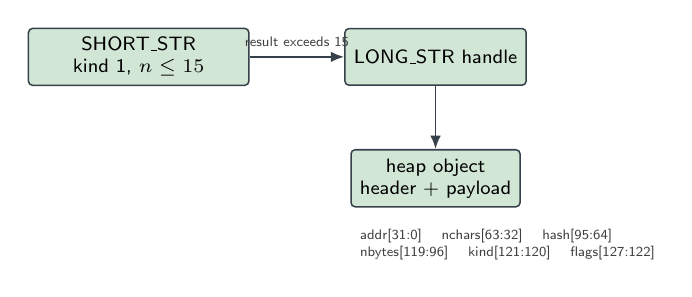
\begin{tikzpicture}[node distance=2mm]
  \node[mem, minimum width=28mm] (short) {SHORT\_STR\\kind 1, $n\le 15$};
  \node[mem, right=12mm of short] (long) {LONG\_STR handle};
  \node[mem, below=8mm of long] (obj) {heap object\\header + payload};
  \draw[arr] (short.east) -- node[anno, above] {result exceeds 15} (long.west);
  \draw[arr] (long) -- (obj);
  \node[anno, align=left, anchor=north west] at ($(obj.south west)+(0,-0.15)$)
    {addr[31:0] \quad nchars[63:32] \quad hash[95:64]\\
     nbytes[119:96] \quad kind[121:120] \quad flags[127:122]};
\end{tikzpicture}
\caption{String representation.
A string is a \texttt{SHORT\_STR} exactly when it is kind~1 (Latin-1) and holds at most 15 characters.
Every other string is a \texttt{LONG\_STR} handle whose payload lives in the object heap.
\texttt{len}, \texttt{hash}, and truthiness read the handle and do not touch memory.
The canonical rule is mandatory in both directions: the accelerator must return a \texttt{SHORT\_STR} for every qualifying result and must not allocate a short \texttt{LONG\_STR}.}
\label{fig:strtag}
\end{figure}


\section{Register stack}
\label{sec:rf}

The operand stack and the locals of every live frame share one 256-entry
ring.
Pointers move; entries do not slide.
A call that does not fit spills a prefix of the ring to data memory and
restores it on return.
The call-frame stack is a third structure and holds only descriptors.

% Register ring, spill, and the call-frame stack. Requires tikz_styles.tex.
\begin{figure}[htbp]
\centering
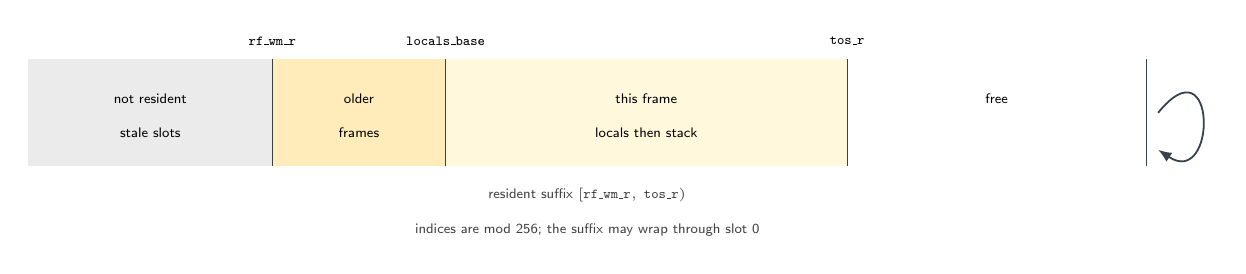
\begin{tikzpicture}[x=1cm,y=1cm]
  % Unwrapped case: tos > wm.
  \draw[pyedge] (0,0) rectangle (14.2,1.35);
  \fill[black!8] (0,0) rectangle (3.1,1.35);
  \fill[pyrf] (3.1,0) rectangle (5.3,1.35);
  \fill[pyhi] (5.3,0) rectangle (10.4,1.35);
  \fill[white] (10.4,0) rectangle (14.2,1.35);
  \draw[pyedge] (3.1,0) -- (3.1,1.35);
  \draw[pyedge] (5.3,0) -- (5.3,1.35);
  \draw[pyedge] (10.4,0) -- (10.4,1.35);
  \node[font=\tiny\sffamily] at (1.55,0.85) {not resident};
  \node[font=\tiny\sffamily] at (1.55,0.42) {stale slots};
  \node[font=\tiny\sffamily] at (4.2,0.85) {older};
  \node[font=\tiny\sffamily] at (4.2,0.42) {frames};
  \node[font=\tiny\sffamily] at (7.85,0.85) {this frame};
  \node[font=\tiny\sffamily] at (7.85,0.42) {locals then stack};
  \node[font=\tiny\sffamily] at (12.3,0.85) {free};
  \node[font=\tiny] at (3.1,1.58) {\texttt{rf\_wm\_r}};
  \node[font=\tiny] at (5.3,1.58) {\texttt{locals\_base}};
  \node[font=\tiny] at (10.4,1.58) {\texttt{tos\_r}};
  \node[anno] at (7.1,-0.38) {resident suffix $[\texttt{rf\_wm\_r},\,\texttt{tos\_r})$};
  \node[anno] at (7.1,-0.82) {indices are mod 256; the suffix may wrap through slot 0};
  \draw[arr] (14.35,0.67) .. controls (15.1,1.6) and (15.1,-0.3) .. (14.35,0.2);
\end{tikzpicture}
\caption{Operand ring, the common case \texttt{tos\_r} $>$ \texttt{rf\_wm\_r}.
The physical file is 256 entries and does not shift.
\texttt{tos\_r} is the next free slot; the top value sits at \texttt{tos\_r}$-1$.
\texttt{locals\_base} is the callee's slot 0.
Frame 0 is an ordinary frame: nothing reserves \texttt{RF[0..31]}.
The three pointers live in \texttt{pycore\_core}.
The regfile module's own push, pop, and TOS ports are tied off.}
\label{fig:ring}
\end{figure}

\begin{figure}[htbp]
\centering
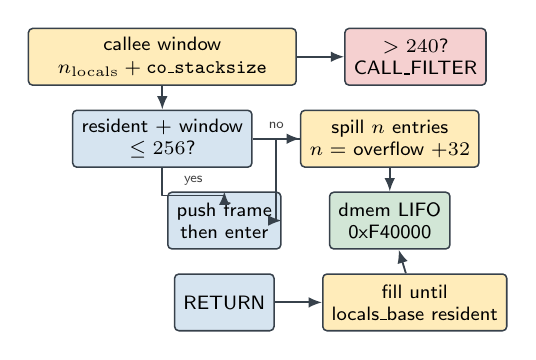
\begin{tikzpicture}[node distance=3mm and 6mm]
  \node[rf, minimum width=34mm] (need) {callee window\\$n_\mathrm{locals}+\texttt{co\_stacksize}$};
  \node[trap, right=of need] (filt) {$> 240$?\\CALL\_FILTER};
  \node[ctl, below=of need] (fit) {resident $+$ window\\$\le 256$?};
  \node[rf, right=of fit] (spill) {spill $n$ entries\\$n =$ overflow $+ 32$};
  \node[mem, below=of spill] (lifo) {dmem LIFO\\0xF40000};
  \node[ctl, left=of lifo] (push) {push frame\\then enter};
  \node[ctl, below=of push] (ret) {RETURN};
  \node[rf, right=of ret] (fill) {fill until\\locals\_base resident};

  \draw[arr] (need) -- (filt);
  \draw[arr] (need) -- (fit);
  \draw[arr] (fit) -- node[anno, above] {no} (spill);
  \draw[arr] (spill) -- (lifo);
  \draw[arr] (fit.south) -- ++(0,-0.35) -| node[anno, pos=0.25, above] {yes} (push.north);
  \draw[arr] (spill.west) -- ++(-0.3,0) |- (push.east);
  \draw[arr] (ret) -- (fill);
  \draw[arr] (fill) -- (lifo);
\end{tikzpicture}
\caption{Spill and fill around a call.
A callee must keep its whole window resident.
The window is capped at \texttt{RF\_WINDOW\_CAP} $= 240$ (256 entries minus a 16-entry reserve); a larger frame is \texttt{CALL\_FILTER}.
If the live suffix plus that window would exceed 256, \texttt{S\_RF\_SPILL} evicts the overflow plus \texttt{RF\_SPILL\_HYST} $= 32$ entries, clamped to the resident count.
Each entry is two 16-byte beats, value then tag, at the spill stack pointer.
\texttt{S\_RF\_FILL} restores them on return until \texttt{locals\_base} is inside the suffix.
Spilling in the middle of a frame is not implemented.}
\label{fig:spill}
\end{figure}

\begin{figure}[htbp]
\centering
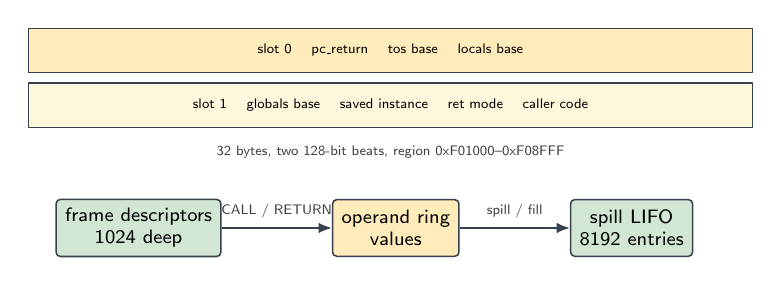
\begin{tikzpicture}[node distance=6mm and 14mm]
  \node[slot, minimum width=92mm, fill=pyrf] (s0)
    {slot 0 \quad pc\_return \quad tos base \quad locals base};
  \node[slot, minimum width=92mm, fill=pyhi, below=1.2mm of s0] (s1)
    {slot 1 \quad globals base \quad saved instance \quad ret mode \quad caller code};
  \node[anno, below=1mm of s1] {32 bytes, two 128-bit beats, region 0xF01000--0xF08FFF};
  \node[mem, below=9mm of s1, xshift=-32mm] (frames) {frame descriptors\\1024 deep};
  \node[rf, right=of frames] (ring) {operand ring\\values};
  \node[mem, right=of ring] (spill) {spill LIFO\\8192 entries};
  \draw[arr] (frames) -- node[anno, above] {CALL / RETURN} (ring);
  \draw[arr] (ring) -- node[anno, above] {spill / fill} (spill);
\end{tikzpicture}
\caption{Three different stacks.
The call frame in \texttt{pycore\_frame} stores pointers, not register values: return PC, TOS base, locals base, globals base, the saved instance, the return-mode bit, and the caller's code-object address.
The operand values stay in the ring.
Values that do not fit the ring move to the spill LIFO at \texttt{0xF40000} (256\,KB).
Return pops slot~1 then slot~0, restores those pointers, and reloads the caller's \texttt{co\_consts} and \texttt{co\_names}.}
\label{fig:frames}
\end{figure}

\begin{figure}[htbp]
\centering
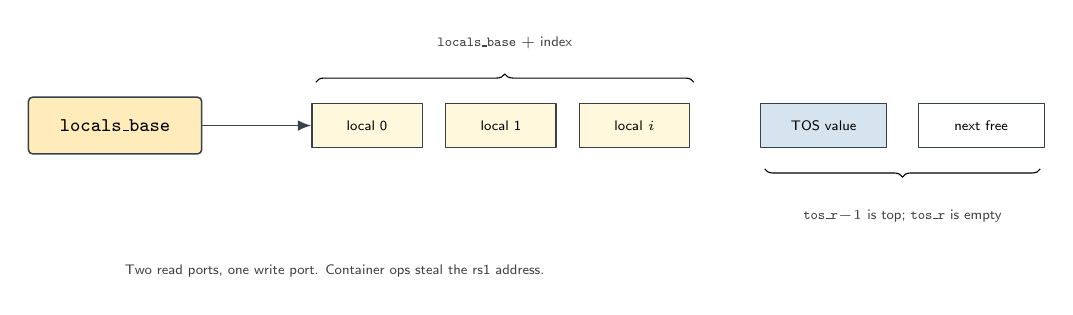
\begin{tikzpicture}[x=1cm,y=1cm]
  \node[rf, minimum width=22mm] (base) at (0,0) {\texttt{locals\_base}};
  \node[slot, fill=pyhi, minimum width=14mm] (l0) at (3.2,0) {local 0};
  \node[slot, fill=pyhi, minimum width=14mm] (l1) at (4.9,0) {local 1};
  \node[slot, fill=pyhi, minimum width=14mm] (lk) at (6.6,0) {local $i$};
  \node[slot, fill=pyctl, minimum width=16mm] (tos1) at (9.0,0) {TOS value};
  \node[slot, fill=white, minimum width=16mm] (tos) at (11.0,0) {next free};
  \draw[arr] (base) -- (l0);
  \draw[decorate, decoration={brace, amplitude=3pt}] (2.55,0.55) -- (7.35,0.55);
  \node[anno] at (4.95,1.05) {\texttt{locals\_base} $+$ index};
  \draw[decorate, decoration={brace, amplitude=3pt, mirror}] (8.25,-0.55) -- (11.75,-0.55);
  \node[anno] at (10.0,-1.15) {\texttt{tos\_r}$-1$ is top; \texttt{tos\_r} is empty};
  \node[anno, anchor=west] at (0,-1.85)
    {Two read ports, one write port. Container ops steal the rs1 address.};
\end{tikzpicture}
\caption{How decode addresses the ring.
\texttt{LOAD\_FAST} $i$ reads \texttt{locals\_base}+$i$.
Stack opcodes read and write relative to \texttt{tos\_r}.
\texttt{S\_WB} commits one entry and applies the stack delta.
Container, return, and spill-fill writeback share that single write port, in that priority.
While \texttt{S\_CONTAINER} runs, rs1 is redirected to \texttt{container\_rf\_addr\_r} so a multi-element build does not need a third read port.
Unbound locals are \texttt{CONTROL/UNINIT}; reading one traps rather than returning leftover bits.}
\label{fig:addr}
\end{figure}


\begin{table}[htbp]
\centering
\caption{Ring and stack parameters (\texttt{pycore\_defs.svh}).}
\label{tab:rf}
\small
\begin{tabular}{@{}llp{0.46\textwidth}@{}}
\toprule
Parameter & Value & Meaning \\
\midrule
\texttt{PYCORE\_RF\_DEPTH} & 256 & Entries in the ring. \\
\texttt{PYCORE\_RF\_RESERVE} & 16 & Entries a callee window may not consume. \\
\texttt{PYCORE\_RF\_WINDOW\_CAP} & 240 & Maximum resident window. Larger is \texttt{CALL\_FILTER}. \\
\texttt{PYCORE\_RF\_SPILL\_HYST} & 32 & Extra entries spilled so the next call does not spill immediately. \\
\texttt{PYCORE\_RF\_INIT\_CHUNK} & 32 & Unfilled locals cleared per \texttt{S\_RF\_INIT} burst. \\
\texttt{PYCORE\_RF\_SPILL\_BASE} & \texttt{0xF40000} & Spill LIFO, 256\,KB, 8192 entries. \\
\texttt{PYCORE\_FRAME\_STACK\_BASE} & \texttt{0xF01000} & Frame descriptors, 32\,KB, 1024 frames. \\
\bottomrule
\end{tabular}
\end{table}

The register file has two combinational read ports and one write port.
\texttt{S\_WB}, container writeback, return writeback, and spill-fill
writeback share the write port.
Container operations may redirect the first read address for the duration
of \texttt{S\_CONTAINER}.
There is no forwarding network because the previous instruction has retired
before decode of the next one reads the file.

\section{Memory system}
\label{sec:mem}

The hart presents two master ports, instruction and data.
Behind them is a modified Harvard hierarchy: split level-1 caches, a unified
inclusive level-2, and a 16\,MB RAM.
The port contract is the one the core was written against when memory was a
single-cycle SRAM, so every cache drops in underneath without retiming the
control machine.

% Memory hierarchy, map, caches, and the dmem mux. Requires tikz_styles.tex.
\begin{figure}[p]
\centering
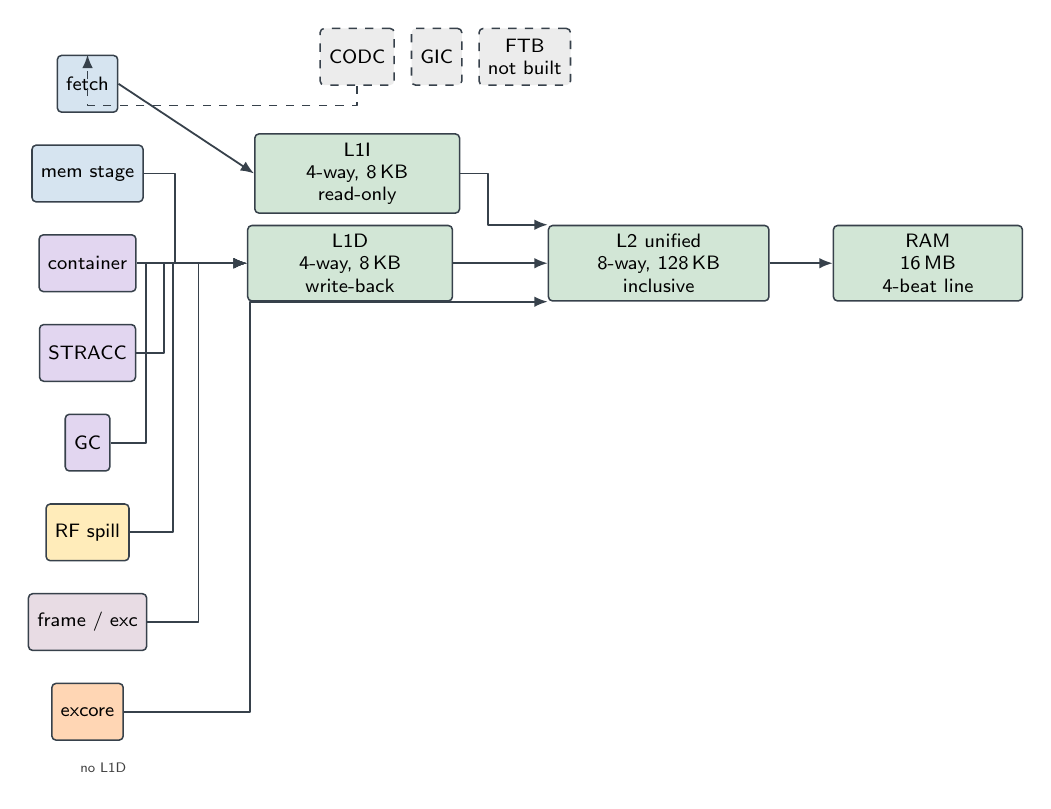
\begin{tikzpicture}[node distance=4mm and 5mm]
  \node[ctl] (fe) {fetch};
  \node[ctl, below=of fe] (ms) {mem stage};
  \node[acc, below=of ms] (cont) {container};
  \node[acc, below=of cont] (sa) {STRACC};
  \node[acc, below=of sa] (gc) {GC};
  \node[rf, below=of gc] (spill) {RF spill};
  \node[ink, below=of spill] (fr) {frame / exc};
  \node[ex, below=of fr] (excore) {excore};

  \node[mem, right=14mm of ms, minimum width=26mm] (l1i) {L1I\\4-way, 8\,KB\\read-only};
  \node[mem, right=14mm of cont, minimum width=26mm] (l1d) {L1D\\4-way, 8\,KB\\write-back};
  \node[mem, right=12mm of l1d, minimum width=28mm] (l2) {L2 unified\\8-way, 128\,KB\\inclusive};
  \node[mem, right=8mm of l2, minimum width=24mm] (ram) {RAM\\16\,MB\\4-beat line};

  \draw[arr] (fe.east) -- (l1i.west);
  \draw[arr] (ms.east) -- ++(0.4,0) |- (l1d.west);
  \draw[arr] (cont.east) -- (l1d.west);
  \draw[arr] (sa.east) -- ++(0.35,0) |- (l1d.west);
  \draw[arr] (gc.east) -- ++(0.45,0) |- (l1d.west);
  \draw[arr] (spill.east) -- ++(0.55,0) |- (l1d.west);
  \draw[arr] (fr.east) -- ++(0.65,0) |- (l1d.west);
  \draw[arr] (l1i.east) -- ++(0.35,0) |- (l2.north west);
  \draw[arr] (l1d.east) -- (l2.west);
  \draw[arr] (l2.east) -- (ram.west);
  \draw[arr] (excore.east) -- ++(1.6,0) |- (l2.south west);

  \node[anno, anchor=north] at ($(excore.south)+(0.2,-0.15)$) {no L1D};
  \node[res, above=6mm of l1i] (codc) {CODC};
  \node[res, right=2mm of codc] (gic) {GIC};
  \node[res, right=2mm of gic, dashed] (ftb) {FTB\\not built};
  \draw[darr] (codc.south) -- ++(0,-0.25) -| (fe.north);
\end{tikzpicture}
\caption{Memory hierarchy behind an unchanged port.
A request is captured on the cycle \texttt{req} is high.
\texttt{ack} pulses for one cycle when the data is ready, any latency later, with \texttt{fault} beside it.
At most one ordinary request is outstanding per master.
\texttt{PYCORE\_CACHE\_EN=0} is a combinational bypass to the next level.
Line size is 64\,B everywhere.
L1 hit latency is 1 cycle; L2 hit latency is 8 cycles (\texttt{PYCORE\_L2\_HIT\_CYCLES}), a model parameter.
The crossbar adds \texttt{PYCORE\_CODE\_ADDR\_BASE} $= \mathtt{0x01000000}$ to instruction addresses so code and data do not alias in L2.
CODC and GIC sit beside the line caches.
The frame-top buffer (\texttt{PYCORE\_FTB\_FRAMES} $= 4$) is a named parameter only.}
\label{fig:hier}
\end{figure}

\begin{figure}[p]
\centering
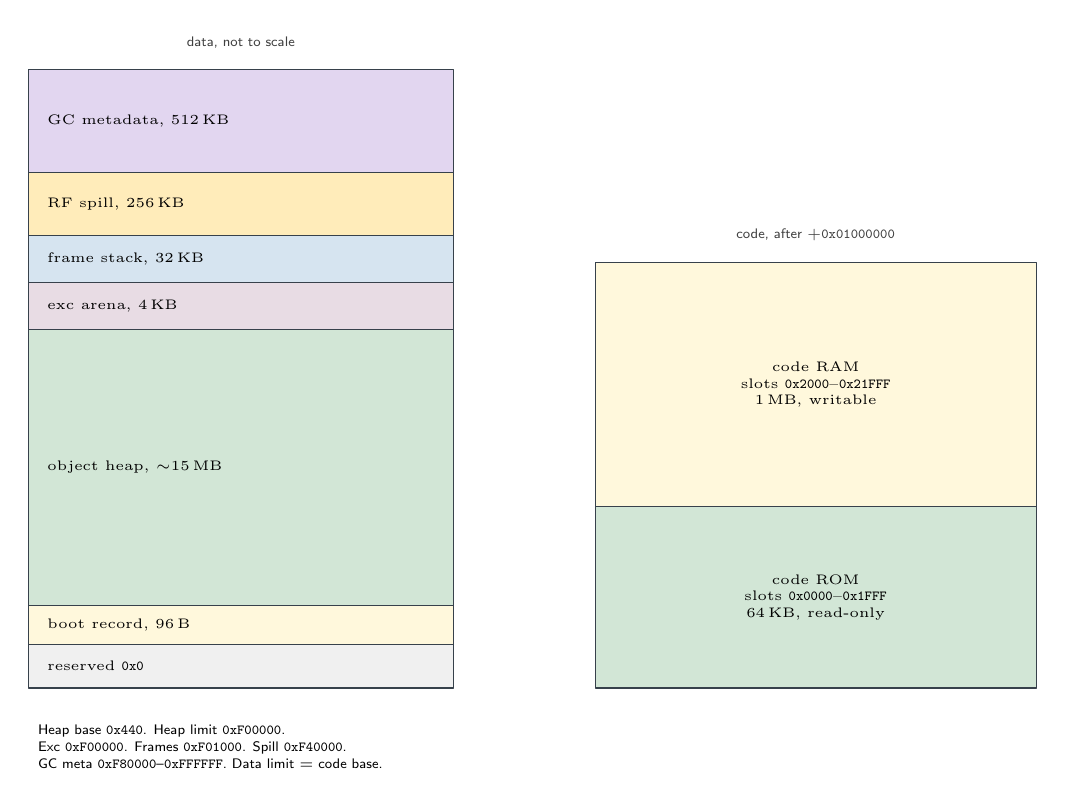
\begin{tikzpicture}[x=1cm,y=1cm]
  % Data map, not to scale. Low addresses at the bottom.
  \begin{scope}[local bounding box=data]
    \fill[black!6] (0,0) rectangle (5.4,0.55);
    \fill[pyhi] (0,0.55) rectangle (5.4,1.05);
    \fill[pymem] (0,1.05) rectangle (5.4,4.55);
    \fill[pyink] (0,4.55) rectangle (5.4,5.15);
    \fill[pyctl] (0,5.15) rectangle (5.4,5.75);
    \fill[pyrf] (0,5.75) rectangle (5.4,6.55);
    \fill[pyacc] (0,6.55) rectangle (5.4,7.85);
    \draw[pyedge] (0,0) rectangle (5.4,7.85);
    \foreach \y in {0.55,1.05,4.55,5.15,5.75,6.55}
      \draw[pyedge] (0,\y) -- (5.4,\y);
    \node[font=\tiny, anchor=west] at (0.12,0.28) {reserved \texttt{0x0}};
    \node[font=\tiny, anchor=west] at (0.12,0.80) {boot record, 96\,B};
    \node[font=\tiny, anchor=west] at (0.12,2.80) {object heap, $\sim$15\,MB};
    \node[font=\tiny, anchor=west] at (0.12,4.85) {exc arena, 4\,KB};
    \node[font=\tiny, anchor=west] at (0.12,5.45) {frame stack, 32\,KB};
    \node[font=\tiny, anchor=west] at (0.12,6.15) {RF spill, 256\,KB};
    \node[font=\tiny, anchor=west] at (0.12,7.20) {GC metadata, 512\,KB};
    \node[anno, anchor=south] at (2.7,8.0) {data, not to scale};
  \end{scope}
  \begin{scope}[xshift=7.2cm, local bounding box=code]
    \fill[pymem] (0,0) rectangle (5.6,2.3);
    \fill[pyhi] (0,2.3) rectangle (5.6,5.4);
    \draw[pyedge] (0,0) rectangle (5.6,5.4);
    \draw[pyedge] (0,2.3) -- (5.6,2.3);
    \node[font=\tiny, align=center] at (2.8,1.15)
      {code ROM\\slots \texttt{0x0000}--\texttt{0x1FFF}\\64\,KB, read-only};
    \node[font=\tiny, align=center] at (2.8,3.85)
      {code RAM\\slots \texttt{0x2000}--\texttt{0x21FFF}\\1\,MB, writable};
    \node[anno, anchor=south] at (2.8,5.55) {code, after $+$\texttt{0x01000000}};
  \end{scope}
  \node[font=\tiny\sffamily, align=left, anchor=north west] at (0,-0.35)
    {Heap base \texttt{0x440}. Heap limit \texttt{0xF00000}.\\
     Exc \texttt{0xF00000}. Frames \texttt{0xF01000}. Spill \texttt{0xF40000}.\\
     GC meta \texttt{0xF80000}--\texttt{0xFFFFFF}. Data limit $=$ code base.};
\end{tikzpicture}
\caption{Address map.
The heap is a bump pointer from \texttt{PYCORE\_HEAP\_BASE} with no free list until the collector is enabled.
The static boot image occupies about 380\,KB of that heap.
Code is a separate slot space: the architectural PC is a slot index, and fetch sends \texttt{pc}$\ll 3$.
\texttt{pycore\_code\_mem} is compiled and not instantiated; the live path is \texttt{pycore\_mem\_hier} into \texttt{pycore\_ram}.}
\label{fig:map}
\end{figure}

\begin{figure}[htbp]
\centering
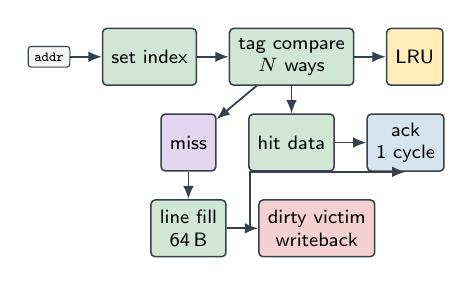
\begin{tikzpicture}[node distance=3.5mm and 4mm]
  \node[bus] (req) {addr};
  \node[mem, right=of req] (idx) {set index};
  \node[mem, right=of idx] (tag) {tag compare\\$N$ ways};
  \node[rf, right=of tag] (lru) {LRU};
  \node[mem, below=of tag] (hit) {hit data};
  \node[acc, left=of hit] (miss) {miss};
  \node[mem, below=of miss] (fill) {line fill\\64\,B};
  \node[trap, right=of fill] (wbv) {dirty victim\\writeback};
  \node[ctl, right=of hit] (ack) {ack\\1 cycle};

  \draw[arr] (req) -- (idx);
  \draw[arr] (idx) -- (tag);
  \draw[arr] (tag) -- (lru);
  \draw[arr] (tag) -- (hit);
  \draw[arr] (tag) -- (miss);
  \draw[arr] (miss) -- (fill);
  \draw[arr] (fill) -- (wbv);
  \draw[arr] (hit) -- (ack);
  \draw[arr] (fill.east) -- ++(0.3,0) |- (ack.south);
\end{tikzpicture}
\caption{One \texttt{pycore\_cache}, three instantiations (L1I, L1D, L2).
L1I is read-only and write-invalidate / no-allocate: a store drops a hit line and forwards the write, and does not allocate.
L1D and L2 are write-back and write-allocate.
An all-zero full-line write on L1D bypasses allocation; STRACC uses full-line installs so a new result line is not filled only to be overwritten.
\texttt{rdata\_line} returns the whole responding line with \texttt{ack}, which is how the fetch buffer fills.}
\label{fig:cache}
\end{figure}

\begin{figure}[htbp]
\centering
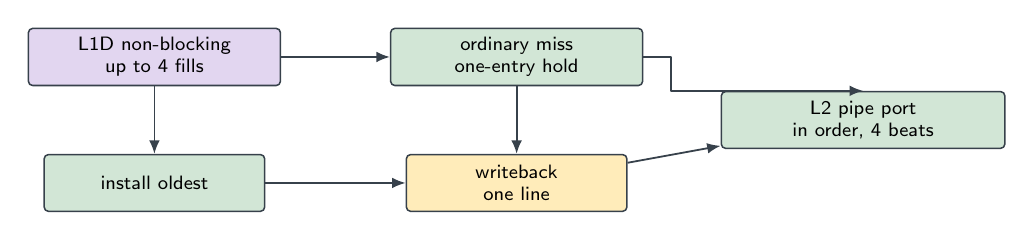
\begin{tikzpicture}[x=1cm,y=1cm]
  \node[acc, minimum width=32mm] (nb) at (0,1.6) {L1D non-blocking\\up to 4 fills};
  \node[mem, minimum width=32mm] (hold) at (4.6,1.6) {ordinary miss\\one-entry hold};
  \node[mem, minimum width=28mm] (inst) at (0,0) {install oldest};
  \node[rf, minimum width=28mm] (wbb) at (4.6,0) {writeback\\one line};
  \node[mem, minimum width=36mm] (pipe) at (9.0,0.8) {L2 pipe port\\in order, 4 beats};
  \draw[arr] (nb) -- (hold);
  \draw[arr] (nb) -- (inst);
  \draw[arr] (inst) -- (wbb);
  \draw[arr] (hold) -- (wbb);
  \draw[arr] (wbb) -- (pipe);
  \draw[arr] (hold.east) -- ++(0.35,0) |- (pipe.north);
\end{tikzpicture}
\caption{The two opt-in ports.
Nothing changes for a master that ignores them: an ordinary request takes the same number of cycles as before.
The collector is the first user.
While marking, it prefetches the line of each object it pushes and the next lines of the range it is scanning.
A prefetch fills L1D and does not produce an answer.}
\label{fig:nb}
\end{figure}

\begin{figure}[htbp]
\centering
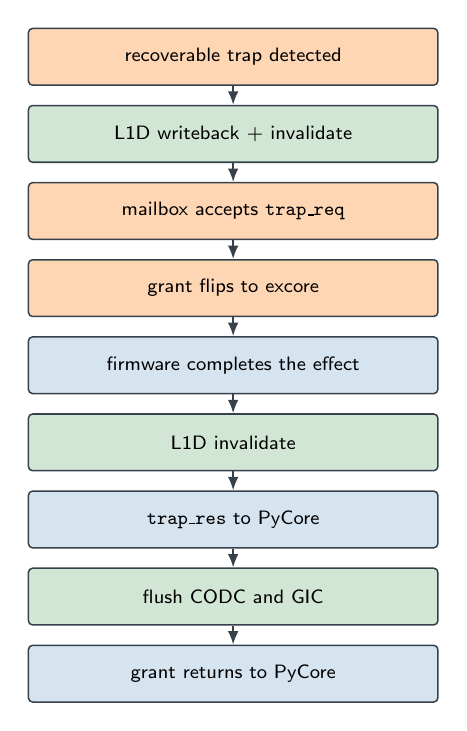
\begin{tikzpicture}[node distance=2.4mm]
  \node[ex, minimum width=52mm] (a) {recoverable trap detected};
  \node[mem, minimum width=52mm, below=of a] (b) {L1D writeback $+$ invalidate};
  \node[ex, minimum width=52mm, below=of b] (c) {mailbox accepts \texttt{trap\_req}};
  \node[ex, minimum width=52mm, below=of c] (d) {grant flips to excore};
  \node[ctl, minimum width=52mm, below=of d] (e) {firmware completes the effect};
  \node[mem, minimum width=52mm, below=of e] (f) {L1D invalidate};
  \node[ctl, minimum width=52mm, below=of f] (g) {\texttt{trap\_res} to PyCore};
  \node[mem, minimum width=52mm, below=of g] (h) {flush CODC and GIC};
  \node[ctl, minimum width=52mm, below=of h] (i) {grant returns to PyCore};
  \foreach \p/\q in {a/b,b/c,c/d,d/e,e/f,f/g,g/h,h/i}
    \draw[arr] (\p) -- (\q);
\end{tikzpicture}
\caption{The only sharing event.
There is no cache coherence protocol.
PyCore issues no data request while excore owns memory, and excore polls the mailbox while PyCore owns it.
L1I is not flushed on the handoff.
L2 is left in place; excore's writes land there and become visible to PyCore after the L1D invalidate.
A code-RAM blit or patch invalidates L1I and flushes CODC.
\texttt{STORE\_NAME} / \texttt{STORE\_GLOBAL} and a change of \texttt{globals\_base\_r} flush the GIC.
A return that restores the same globals base does not.}
\label{fig:handoff}
\end{figure}

\begin{figure}[htbp]
\centering
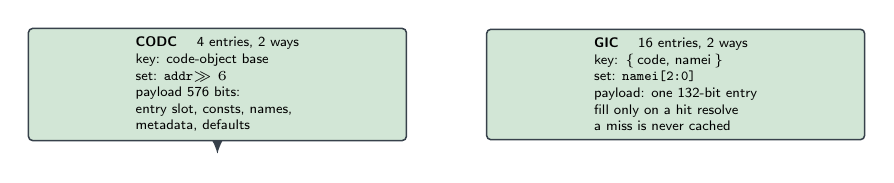
\begin{tikzpicture}[node distance=3mm and 10mm]
  \node[mem, minimum width=48mm, align=left, font=\tiny\sffamily] (codc)
    {\textbf{CODC} \quad 4 entries, 2 ways\\
     key: code-object base\\
     set: \texttt{addr}$\gg 6$\\
     payload 576 bits:\\
     entry slot, consts, names,\\
     metadata, defaults};
  \node[mem, minimum width=48mm, align=left, font=\tiny\sffamily, right=of codc] (gic)
    {\textbf{GIC} \quad 16 entries, 2 ways\\
     key: \{\,code, namei\,\}\\
     set: \texttt{namei[2:0]}\\
     payload: one 132-bit entry\\
     fill only on a hit resolve\\
     a miss is never cached};
  \draw[darr] ($(codc.south)+(0,-0.15)$) -- ++(0,-0.01);
\end{tikzpicture}
\caption{Result caches.
Both answer in the same cycle as the lookup.
Fill and LRU update on the following clock edge.
\texttt{CACHE\_EN=0} forces a miss.
CODC is flushed on \texttt{MAKE\_FUNCTION}, code release, \texttt{trap\_res}, and reset.
The GIC is flushed as a whole on purpose: consulting a dict version to do better would itself be a data-memory access.}
\label{fig:resultcache}
\end{figure}

\begin{figure}[htbp]
\centering
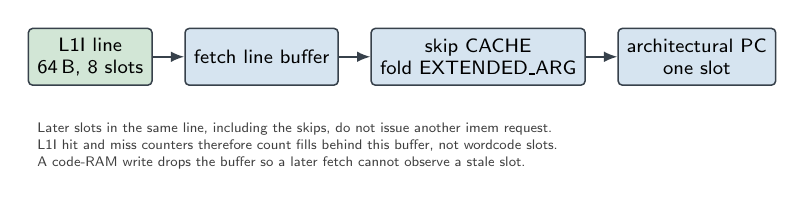
\begin{tikzpicture}[node distance=3.5mm and 4mm]
  \node[mem] (l1i) {L1I line\\64\,B, 8 slots};
  \node[ctl, right=of l1i] (buf) {fetch line buffer};
  \node[ctl, right=of buf] (fold) {skip CACHE\\fold EXTENDED\_ARG};
  \node[ctl, right=of fold] (pc) {architectural PC\\one slot};
  \draw[arr] (l1i) -- (buf);
  \draw[arr] (buf) -- (fold);
  \draw[arr] (fold) -- (pc);
  \node[anno, align=left, anchor=north west] at ($(l1i.south west)+(0,-0.35)$)
    {Later slots in the same line, including the skips, do not issue another imem request.\\
     L1I hit and miss counters therefore count fills behind this buffer, not wordcode slots.\\
     A code-RAM write drops the buffer so a later fetch cannot observe a stale slot.};
\end{tikzpicture}
\caption{Fetch.
The image keeps CPython's \texttt{CACHE} and \texttt{EXTENDED\_ARG} bytes.
The slot index equals the CPython code-unit index, so branch arguments are not rewritten.
The live code image is ROM plus RAM in the unified RAM, selected by the slot address.}
\label{fig:fetch}
\end{figure}

\begin{figure}[htbp]
\centering
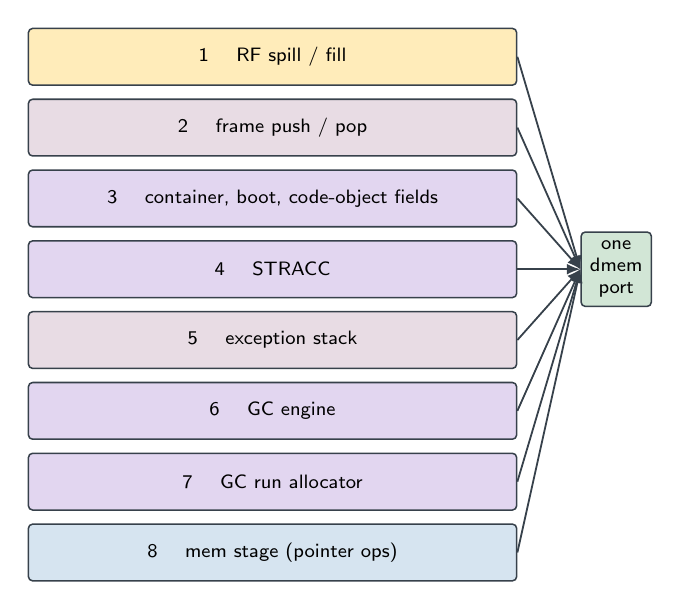
\begin{tikzpicture}[node distance=1.6mm]
  \node[rf, minimum width=62mm] (s1) {1 \quad RF spill / fill};
  \node[ink, minimum width=62mm, below=of s1] (s2) {2 \quad frame push / pop};
  \node[acc, minimum width=62mm, below=of s2] (s3) {3 \quad container, boot, code-object fields};
  \node[acc, minimum width=62mm, below=of s3] (s4) {4 \quad STRACC};
  \node[ink, minimum width=62mm, below=of s4] (s5) {5 \quad exception stack};
  \node[acc, minimum width=62mm, below=of s5] (s6) {6 \quad GC engine};
  \node[acc, minimum width=62mm, below=of s6] (s7) {7 \quad GC run allocator};
  \node[ctl, minimum width=62mm, below=of s7] (s8) {8 \quad mem stage (pointer ops)};
  \node[mem, right=8mm of s4] (port) {one\\dmem\\port};
  \foreach \n in {s1,s2,s3,s4,s5,s6,s7,s8}
    \draw[arr] (\n.east) -- (port.west);
\end{tikzpicture}
\caption{Who drives the data port.
The mux is a priority encode, but the owners are mutually exclusive by core state.
PyCore never arbitrates two live masters in one cycle.
The port is 128-bit data, 16-byte aligned, with a 16-bit write strobe.
A misaligned or out-of-range access raises \texttt{ADDR\_ALIGN} or \texttt{MEM\_FAULT}.
GC also has the non-blocking prefetch port into L1D, which is not this mux.}
\label{fig:dmux}
\end{figure}


\begin{table}[htbp]
\centering
\caption{Line caches. Hit latencies are model parameters.}
\label{tab:caches}
\small
\begin{tabular}{@{}lrrllp{0.28\textwidth}@{}}
\toprule
Level & Size & Ways & Line & Hit & Policy \\
\midrule
L1I & 8\,KB & 4 & 64\,B & 1 & read-only, write-invalidate \\
L1D & 8\,KB & 4 & 64\,B & 1 & write-back, write-allocate, LRU \\
L2 & 128\,KB & 8 & 64\,B & 8 & unified, inclusive, write-back \\
RAM & 16\,MB & --- & 64\,B & --- & 4 beats; CI latency 4 \\
\bottomrule
\end{tabular}
\end{table}

Data width on the CPU side of L1D is 128 bits with a 16-bit strobe.
Instruction width is 64 bits, one slot.
A 64-byte line is four data beats.

\section{Accelerators}
\label{sec:accel}

An accelerator here is any unit that gives a bytecode operation a datapath
shorter than a firmware trap.
They fall into three places, drawn together in Figure~\ref{fig:accel-all}
and then one at a time.

\begin{enumerate}
\item The execute fabric, inside \texttt{S\_EXEC}: integer ALU, multiplier,
      divider, integer power, and the FPU.
\item Port-owning engines that freeze the core: the string accelerator and
      the collector, plus the container FSM, which is microcoded in the
      core rather than a separate module.
\item Excore, for the grow and bulk-update cases the container FSM raises
      before it has committed anything.
\end{enumerate}

% Accelerator map, execute fabric, handshake, integer units.
% Requires tikz_styles.tex.
\begin{figure}[p]
\centering
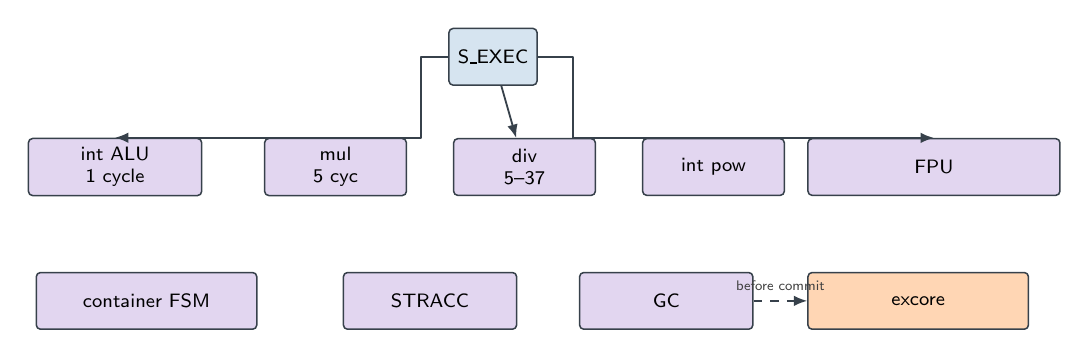
\begin{tikzpicture}[x=1cm,y=1cm]
  \node[ctl] (exec) at (6.2,3.55) {S\_EXEC};
  \node[acc, minimum width=22mm] (alu) at (1.4,2.15) {int ALU\\1 cycle};
  \node[acc, minimum width=18mm] (mul) at (4.2,2.15) {mul\\5 cyc};
  \node[acc, minimum width=18mm] (div) at (6.6,2.15) {div\\5--37};
  \node[acc, minimum width=18mm] (ipow) at (9.0,2.15) {int pow};
  \node[acc, minimum width=32mm] (fpu) at (11.8,2.15) {FPU};
  \node[acc, minimum width=28mm] (cont) at (1.8,0.45) {container FSM};
  \node[acc, minimum width=22mm] (sa) at (5.4,0.45) {STRACC};
  \node[acc, minimum width=22mm] (gc) at (8.4,0.45) {GC};
  \node[ex, minimum width=28mm] (excore) at (11.6,0.45) {excore};
  \draw[arr] (exec) -- (div);
  \draw[arr] (exec.west) -- ++(-0.35,0) |- (alu.north);
  \draw[arr] (exec.east) -- ++(0.45,0) |- (fpu.north);
  \draw[darr] (gc.east) -- node[anno, above] {before commit} (excore.west);
\end{tikzpicture}
\caption{Accelerators, together.
Three kinds of hardware sit off the simple pipeline.
The execute fabric is tag-routed arithmetic and stays inside \texttt{S\_EXEC}.
The container FSM, the string accelerator, and the collector are multi-cycle masters of the data port; the core is frozen in their state until they finish.
Excore is the firmware accelerator for the cases those units refuse to do in place: growing a container and the uncontaminated bulk updates.
Negative integer powers never reach the integer power unit; execute promotes both operands and reissues them on the FPU.}
\label{fig:accel-all}
\end{figure}

\begin{figure}[p]
\centering
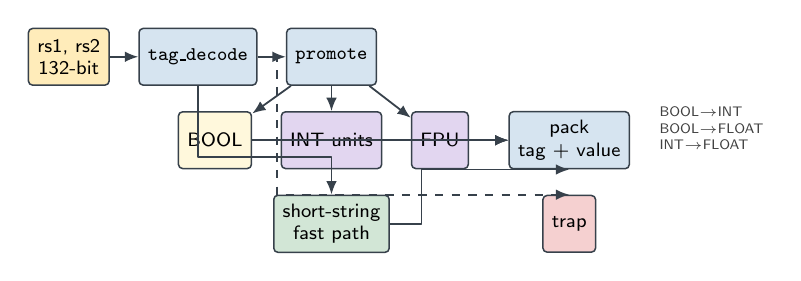
\begin{tikzpicture}[node distance=3.2mm and 3.6mm]
  \node[rf] (rs) {rs1, rs2\\132-bit};
  \node[ctl, right=of rs] (td) {\texttt{tag\_decode}};
  \node[ctl, right=of td] (pr) {\texttt{promote}};
  \node[acc, below=of pr] (intu) {INT units};
  \node[acc, right=of intu] (fpu) {FPU};
  \node[hi, left=of intu] (bool) {BOOL};
  \node[mem, below=of intu] (str) {short-string\\fast path};
  \node[ctl, right=5mm of fpu] (pack) {pack\\tag $+$ value};
  \node[trap, below=of pack] (tr) {trap};
  \draw[arr] (rs) -- (td);
  \draw[arr] (td) -- (pr);
  \draw[arr] (pr) -- (intu);
  \draw[arr] (pr) -- (fpu);
  \draw[arr] (pr) -- (bool);
  \draw[arr] (td.south) -- ++(0,-0.9) -| (str.north);
  \draw[arr] (intu) -- (pack);
  \draw[arr] (fpu) -- (pack);
  \draw[arr] (bool.east) -- ++(0.3,0) |- (pack.west);
  \draw[arr] (str.east) -- ++(0.4,0) |- (pack.south);
  \draw[darr] (td.east) -- ++(0.25,0) |- (tr.north);
  \node[anno, anchor=west, align=left] at ($(pack.east)+(0.25,0.15)$)
    {BOOL$\to$INT\\BOOL$\to$FLOAT\\INT$\to$FLOAT};
\end{tikzpicture}
\caption{Execute fabric (\texttt{pycore\_exec}).
Tag decode chooses the unit, the promotion, and the result tag.
Promotion is a combinational rewrite of the 64-bit lane.
The integer ALU, BOOL operations, short-string compare and concatenation, and the FPU's compares and unary operations finish in the issue cycle.
Multiplier, divider, integer power, and the FPU hold \texttt{S\_EXEC} through \texttt{stall\_o}.
The result is written back as a fresh 132-bit entry.
An integer result is sign-extended from 64 bits into the high half.}
\label{fig:exec}
\end{figure}

\begin{figure}[htbp]
\centering
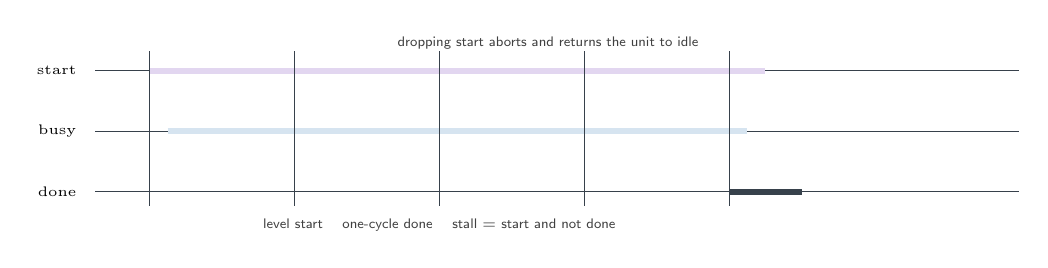
\begin{tikzpicture}[x=1.15cm,y=0.7cm]
  \draw[pyedge] (0,2.2) -- (10.2,2.2);
  \draw[pyedge] (0,1.1) -- (10.2,1.1);
  \draw[pyedge] (0,0) -- (10.2,0);
  \node[anchor=east, font=\tiny] at (-0.1,2.2) {start};
  \node[anchor=east, font=\tiny] at (-0.1,1.1) {busy};
  \node[anchor=east, font=\tiny] at (-0.1,0) {done};
  \draw[pyacc, line width=2.2pt] (0.6,2.2) -- (7.4,2.2);
  \draw[pyctl, line width=2.2pt] (0.8,1.1) -- (7.2,1.1);
  \draw[pyedge, line width=2.2pt] (7.0,0) -- (7.8,0);
  \foreach \x in {0.6,2.2,3.8,5.4,7.0} {
    \draw[pyedge, thin] (\x,-0.25) -- (\x,2.55);
  }
  \node[anno] at (3.8,-0.6) {level start \quad one-cycle done \quad stall $=$ start and not done};
  \node[anno] at (5.0,2.7) {dropping start aborts and returns the unit to idle};
\end{tikzpicture}
\caption{Shared handshake of every multi-cycle arithmetic unit.
\texttt{start} is a level.
The unit accepts it when idle and not already in the done cycle, so a requester that holds \texttt{start} and swaps operands the cycle after \texttt{done} gets back-to-back issue.
\texttt{busy} is the structural-hazard bit a later scoreboard would use.
Traps (\texttt{div\_zero}, integer overflow, FPU exception) replace \texttt{done} and are reported with \texttt{stall} low.
The core leaves \texttt{S\_EXEC} by dropping \texttt{start}, which is what aborts a unit today.}
\label{fig:hs}
\end{figure}

\begin{figure}[htbp]
\centering
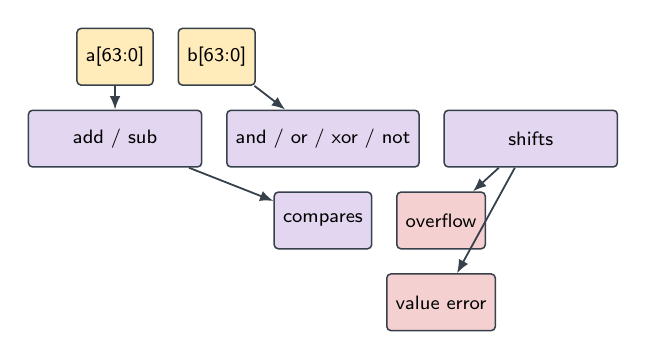
\begin{tikzpicture}[node distance=3mm and 3mm]
  \node[rf] (a) {a[63:0]};
  \node[rf, right=of a] (b) {b[63:0]};
  \node[acc, below=of a, minimum width=22mm] (add) {add / sub};
  \node[acc, right=of add, minimum width=22mm] (log) {and / or / xor / not};
  \node[acc, right=of log, minimum width=22mm] (sh) {shifts};
  \node[acc, below=of log] (cmp) {compares};
  \node[trap, right=of cmp] (ov) {overflow};
  \node[trap, below=of ov] (ve) {value error};
  \draw[arr] (a) -- (add);
  \draw[arr] (b) -- (log);
  \draw[arr] (add) -- (cmp);
  \draw[arr] (sh) -- (ov);
  \draw[arr] (sh) -- (ve);
\end{tikzpicture}
\caption{Integer ALU (\texttt{pycore\_int\_alu}), combinational in the issue cycle.
It covers \texttt{+ - << >> \& | \textasciicircum\ \textasciitilde}, unary plus and minus, and the integer compares.
Beside the result it reports two flags.
\texttt{overflow\_flag} is set when add, subtract, unary minus, or a shift leaves the signed 64-bit range.
\texttt{value\_error} is a negative shift count.
Execute turns those into \texttt{PY\_TRAP\_OVERFLOW} and \texttt{PY\_TRAP\_VALUE}.
Compares reuse the subtractor and ignore the overflow flag.
A shift of 64 or more is the sign fill for \texttt{>>}, and either zero or overflow for \texttt{<<}, matching CPython's long-shift rules on a 64-bit limb.}
\label{fig:alu}
\end{figure}

\begin{figure}[htbp]
\centering
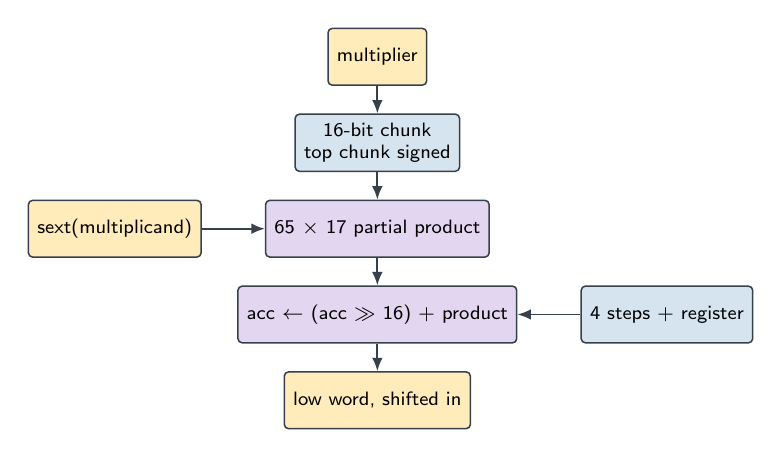
\begin{tikzpicture}[node distance=3.5mm]
  \node[rf] (b) {multiplier};
  \node[ctl, below=of b] (ch) {16-bit chunk\\top chunk signed};
  \node[acc, below=of ch] (pp) {65 $\times$ 17 partial product};
  \node[rf, left=8mm of pp] (a) {sext(multiplicand)};
  \node[acc, below=of pp] (acc) {acc $\leftarrow$ (acc $\gg$ 16) $+$ product};
  \node[rf, below=of acc] (lo) {low word, shifted in};
  \node[ctl, right=8mm of acc] (n) {4 steps $+$ register};
  \draw[arr] (b) -- (ch);
  \draw[arr] (ch) -- (pp);
  \draw[arr] (a) -- (pp);
  \draw[arr] (pp) -- (acc);
  \draw[arr] (acc) -- (lo);
  \draw[arr] (n) -- (acc);
\end{tikzpicture}
\caption{Signed 64$\times$64 multiplier (\texttt{pycore\_mul}, \texttt{STEP}$=16$).
Each cycle multiplies the full multiplicand by one chunk of the multiplier and folds it into a shift-right accumulator.
The multiplier is treated as unsigned chunks with only the top chunk signed, so the running sum is the exact signed product with no final correction.
Four steps plus the registered result are 5 cycles.
The low 64 bits are the Python product when it fits; a high half that is not the sign extension of the low half is \texttt{PY\_TRAP\_OVERFLOW}.
The same multiplier is the engine behind integer power.
\texttt{STEP} is the area-versus-latency knob; the rest of the core does not depend on it.}
\label{fig:mul}
\end{figure}

\begin{figure}[htbp]
\centering
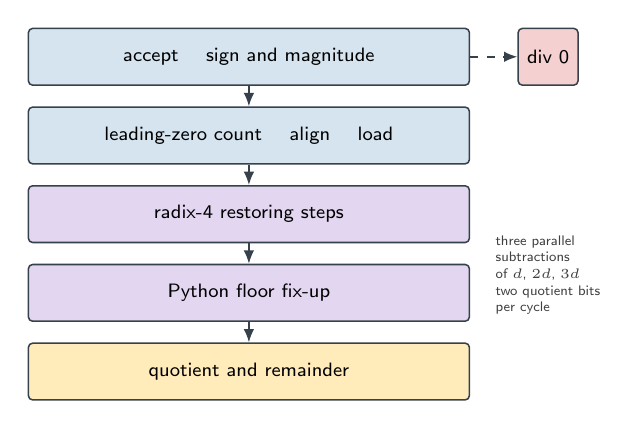
\begin{tikzpicture}[node distance=2.6mm]
  \node[ctl, minimum width=56mm] (c0) {accept \quad sign and magnitude};
  \node[ctl, minimum width=56mm, below=of c0] (c1) {leading-zero count \quad align \quad load};
  \node[acc, minimum width=56mm, below=of c1] (run) {radix-4 restoring steps};
  \node[acc, minimum width=56mm, below=of run] (fix) {Python floor fix-up};
  \node[rf, minimum width=56mm, below=of fix] (out) {quotient and remainder};
  \node[trap, right=6mm of c0] (z) {div 0};
  \foreach \p/\q in {c0/c1,c1/run,run/fix,fix/out} \draw[arr] (\p) -- (\q);
  \draw[darr] (c0) -- (z);
  \node[anno, align=left, anchor=north west] at ($(run.east)+(0.2,-0.15)$)
    {three parallel\\subtractions\\of $d$, $2d$, $3d$\\two quotient bits\\per cycle};
\end{tikzpicture}
\caption{Floor divider (\texttt{pycore\_div}, \texttt{RL}$=2$) on \texttt{pycore\_udiv\_seq}.
Only $n = \mathrm{bits}(|a|) - \mathrm{bits}(|b|) + 1$ quotient bits are iterated, rounded up to a multiple of two.
Latency is $5 + \lceil n/2 \rceil$: 5 cycles when $|a| < |b|$, 37 for a full 64-bit quotient.
The five fixed cycles are accept, leading-zero and alignment, core load, core result, and the floor fix-up.
Division by zero is combinational in the accept cycle and does not start the unit.
\texttt{INT64\_MIN // -1} overflows.
The same restoring core with \texttt{SQRT}$=1$ is the floating-point square root.}
\label{fig:div}
\end{figure}

\begin{figure}[htbp]
\centering
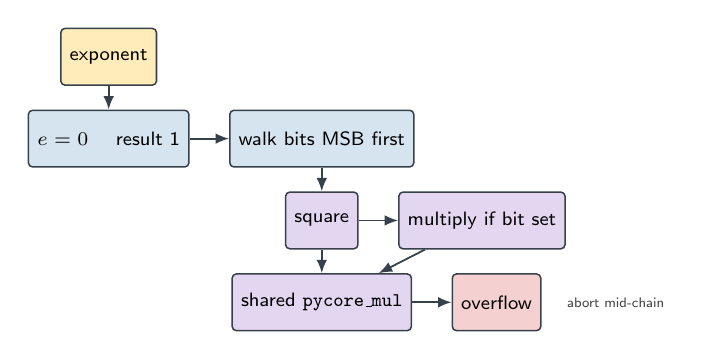
\begin{tikzpicture}[node distance=3mm and 5mm]
  \node[rf] (e) {exponent};
  \node[ctl, below=of e] (z) {$e = 0$ \quad result 1};
  \node[ctl, right=of z] (bits) {walk bits MSB first};
  \node[acc, below=of bits] (sq) {square};
  \node[acc, right=of sq] (mu) {multiply if bit set};
  \node[acc, below=of sq] (mul) {shared \texttt{pycore\_mul}};
  \node[trap, right=of mul] (ov) {overflow};
  \draw[arr] (e) -- (z);
  \draw[arr] (z) -- (bits);
  \draw[arr] (bits) -- (sq);
  \draw[arr] (sq) -- (mu);
  \draw[arr] (sq) -- (mul);
  \draw[arr] (mu) -- (mul);
  \draw[arr] (mul) -- (ov);
  \node[anno, anchor=west] at ($(ov.east)+(0.2,0)$) {abort mid-chain};
\end{tikzpicture}
\caption{Integer power (\texttt{pycore\_ipow}).
A non-negative exponent does $\mathrm{bits}(e)-1$ squarings and $\mathrm{popcount}(e)-1$ extra multiplies, each a full multiplier pass, plus four cycles of sequencing.
A zero exponent finishes in the issue cycle.
A negative exponent is a float in Python and is re-routed before this unit.
The unit traps as soon as an intermediate product leaves the signed 64-bit range, so the long chains that complete are bases $0$, $1$, and $-1$.}
\label{fig:ipow}
\end{figure}


\begin{table}[htbp]
\centering
\caption{Arithmetic latency, in cycles, counting the accept cycle.
Divider latency depends on the number of quotient bits $n$.
Integer power does $k = \mathrm{bits}(e)-1$ squarings and
$p = \mathrm{popcount}(e)-1$ extra multiplies.}
\label{tab:lat}
\small
\begin{tabular}{@{}llr@{}}
\toprule
Unit & Operation & Cycles \\
\midrule
\texttt{pycore\_int\_alu} & add, logic, shift, compare & 1 \\
\texttt{pycore\_mul} & 64$\times$64 signed, step 16 & 5 \\
\texttt{pycore\_div} & floor division and remainder & $5 + \lceil n/2 \rceil$ \\
\texttt{pycore\_ipow} & non-negative integer power & $4 + 6k + 5p$ \\
\texttt{pycore\_fp\_add} & binary64 add / sub & 4 \\
\texttt{pycore\_fp\_mul} & binary64 multiply & 6 \\
\texttt{pycore\_fp\_divrem} & binary64 divide or square root & 32 \\
\texttt{pycore\_fp\_divrem} & \texttt{fmod}, exponent gap $d \ge 0$ & $5 + \lceil(d+1)/2\rceil$ \\
\texttt{pycore\_fp\_pow} & general binary64 power & 166 \\
\texttt{pycore\_fpu} & general \texttt{float ** float} & 171 \\
\texttt{pycore\_fpu} & complex add / mul / div & 10 / 34 / 128 \\
\bottomrule
\end{tabular}
\end{table}

\texttt{NB\_TRUE\_DIVIDE} always yields \texttt{FLOAT}, including
\texttt{INT / INT}: both operands are converted to binary64 before the
divider.
\texttt{INT ** INT} with a negative exponent takes that same floating-point
path.
A negative base with a fractional exponent traps; the FPU has no complex power.

\subsection{Floating point}

% FPU sequencer and the four floating-point datapaths.
% Requires tikz_styles.tex.
\begin{figure}[p]
\centering
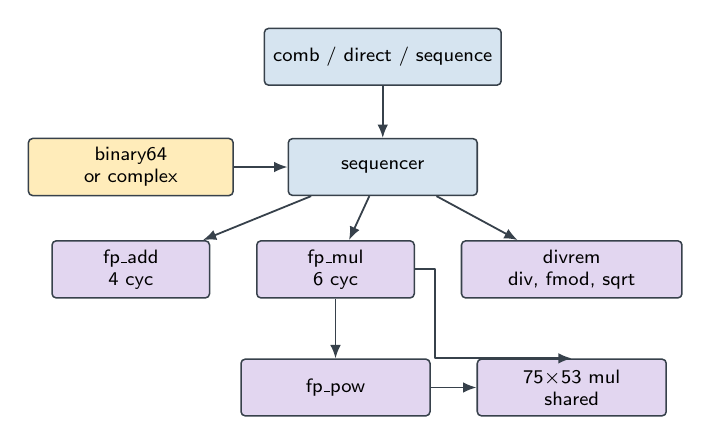
\begin{tikzpicture}[x=1cm,y=1cm]
  \node[rf, minimum width=26mm] (ops) at (0,1.3) {binary64\\or complex};
  \node[ctl, minimum width=24mm] (seq) at (3.2,1.3) {sequencer};
  \node[ctl, minimum width=28mm] (kind) at (3.2,2.7) {comb / direct / sequence};
  \node[acc, minimum width=20mm] (add) at (0,0) {fp\_add\\4 cyc};
  \node[acc, minimum width=20mm] (mul) at (2.6,0) {fp\_mul\\6 cyc};
  \node[acc, minimum width=28mm] (div) at (5.6,0) {divrem\\div, fmod, sqrt};
  \node[acc, minimum width=24mm] (pow) at (2.6,-1.5) {fp\_pow};
  \node[acc, minimum width=24mm] (um) at (5.6,-1.5) {75$\times$53 mul\\shared};
  \draw[arr] (ops) -- (seq);
  \draw[arr] (kind) -- (seq);
  \draw[arr] (seq) -- (add);
  \draw[arr] (seq) -- (mul);
  \draw[arr] (seq) -- (div);
  \draw[arr] (mul) -- (pow);
  \draw[arr] (mul.east) -- ++(0.25,0) |- (um.north);
  \draw[arr] (pow) -- (um);
\end{tikzpicture}
\caption{FPU (\texttt{pycore\_fpu}).
One adder, one multiplier, one divider, and one power unit.
The divider is also the square root.
The significand multiplier is a single \texttt{pycore\_umul\_seq} of 75$\times$53, step 14, muxed between \texttt{fp\_mul} (53$\times$53, zero-extended) and \texttt{fp\_pow}.
The sequencer never runs those two at once.
Scalar add, subtract, multiply, and divide pass through.
Remainder, floor division, general powers, and complex arithmetic are sequences of those datapaths in CPython's order.
Compares, \texttt{not}, and unary plus and minus are combinational.}
\label{fig:fpu}
\end{figure}

\begin{figure}[htbp]
\centering
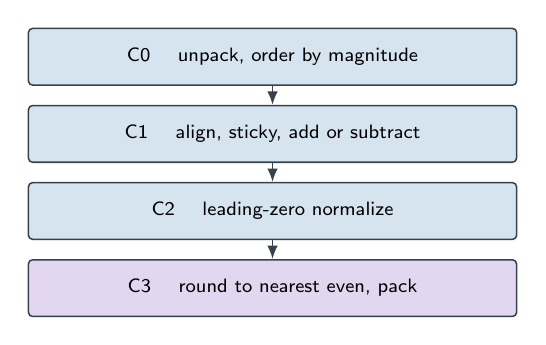
\begin{tikzpicture}[node distance=2.4mm]
  \node[ctl, minimum width=62mm] (c0) {C0 \quad unpack, order by magnitude};
  \node[ctl, minimum width=62mm, below=of c0] (c1) {C1 \quad align, sticky, add or subtract};
  \node[ctl, minimum width=62mm, below=of c1] (c2) {C2 \quad leading-zero normalize};
  \node[acc, minimum width=62mm, below=of c2] (c3) {C3 \quad round to nearest even, pack};
  \foreach \p/\q in {c0/c1,c1/c2,c2/c3} \draw[arr] (\p) -- (\q);
\end{tikzpicture}
\caption{Binary64 add and subtract (\texttt{pycore\_fp\_add}).
Three registered stages; the round and pack of the last stage are combinational, so \texttt{done} is four cycles after accept.
Specials (NaN, infinity) can be decided in C0 and carried forward.
Subnormals, signed zeros, and the guard/round/sticky scheme are in the shared packer \texttt{pycore\_f64\_pack\_round}.
Each stage already has its own valid bit so the unit can later accept a new operation while an old one drains.}
\label{fig:fpadd}
\end{figure}

\begin{figure}[htbp]
\centering
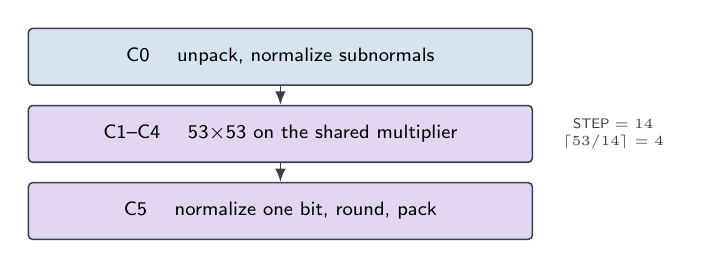
\begin{tikzpicture}[node distance=2.4mm]
  \node[ctl, minimum width=64mm] (c0) {C0 \quad unpack, normalize subnormals};
  \node[acc, minimum width=64mm, below=of c0] (st) {C1--C4 \quad 53$\times$53 on the shared multiplier};
  \node[acc, minimum width=64mm, below=of st] (pk) {C5 \quad normalize one bit, round, pack};
  \foreach \p/\q in {c0/st,st/pk} \draw[arr] (\p) -- (\q);
  \node[anno, anchor=west] at ($(st.east)+(0.25,0)$) {STEP $= 14$\\$\lceil 53/14\rceil = 4$};
\end{tikzpicture}
\caption{Binary64 multiply (\texttt{pycore\_fp\_mul}).
The 53$\times$53 significand product is iterative.
At the default step, \texttt{done} is the sixth cycle counting accept as the first.
The parent owns the multiplier; this unit only presents operands and waits for the product.}
\label{fig:fpmul}
\end{figure}

\begin{figure}[htbp]
\centering
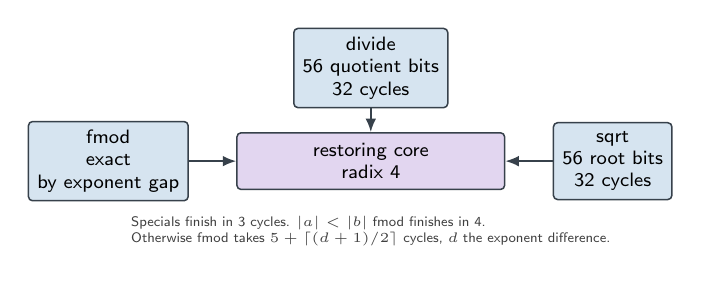
\begin{tikzpicture}[node distance=3mm and 6mm]
  \node[acc, minimum width=34mm] (divu) {restoring core\\radix 4};
  \node[ctl, above=of divu] (div) {divide\\56 quotient bits\\32 cycles};
  \node[ctl, left=of divu] (fmod) {fmod\\exact\\by exponent gap};
  \node[ctl, right=of divu] (sqrt) {sqrt\\56 root bits\\32 cycles};
  \draw[arr] (div) -- (divu);
  \draw[arr] (fmod) -- (divu);
  \draw[arr] (sqrt) -- (divu);
  \node[anno, align=left, anchor=north] at ($(divu.south)+(0,-0.2)$)
    {Specials finish in 3 cycles. $|a|<|b|$ fmod finishes in 4.\\
     Otherwise fmod takes $5+\lceil(d+1)/2\rceil$ cycles, $d$ the exponent difference.};
\end{tikzpicture}
\caption{Divider, remainder, and square root (\texttt{pycore\_fp\_divrem} on \texttt{pycore\_udiv\_seq}).
Division iterates 56 quotient bits, two per cycle.
Square root uses the same remainder register and the same three subtractors, with the divisor multiples replaced by the root-digit candidates $q(8Q+q)$ for $q \in \{1,2,3\}$.
The final remainder is the sticky bit, so the root is correctly rounded.
The sequencer sends $x^{0.5}$ here (35 cycles including the power special-case setup) instead of through the general power unit.}
\label{fig:fpdiv}
\end{figure}

\begin{figure}[p]
\centering
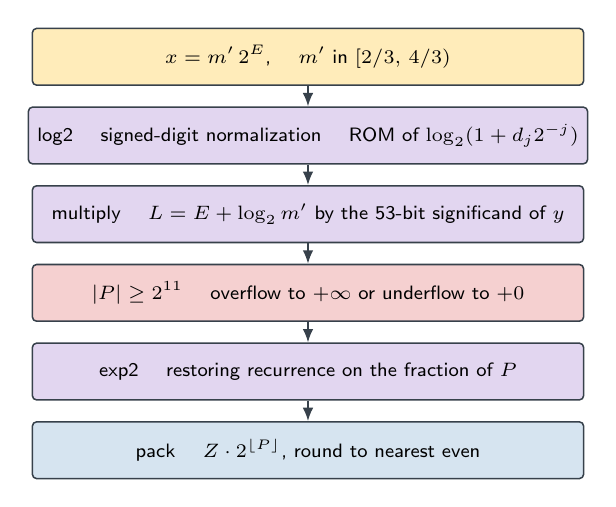
\begin{tikzpicture}[node distance=2.6mm]
  \node[rf, minimum width=70mm] (in) {$x = m'\,2^{E}$, \quad $m'$ in $[2/3,\,4/3)$};
  \node[acc, minimum width=70mm, below=of in] (log)
    {log2 \quad signed-digit normalization \quad ROM of $\log_2(1+d_j 2^{-j})$};
  \node[acc, minimum width=70mm, below=of log] (mul)
    {multiply \quad $L = E + \log_2 m'$ by the 53-bit significand of $y$};
  \node[trap, minimum width=70mm, below=of mul] (lim)
    {$|P| \ge 2^{11}$ \quad overflow to $+\infty$ or underflow to $+0$};
  \node[acc, minimum width=70mm, below=of lim] (exp)
    {exp2 \quad restoring recurrence on the fraction of $P$};
  \node[ctl, minimum width=70mm, below=of exp] (pk)
    {pack \quad $Z \cdot 2^{\lfloor P \rfloor}$, round to nearest even};
  \foreach \p/\q in {in/log,log/mul,mul/lim,lim/exp,exp/pk} \draw[arr] (\p) -- (\q);
\end{tikzpicture}
\caption{Binary64 power (\texttt{pycore\_fp\_pow}): $x^{y} = 2^{y \log_2 x}$ for positive finite $x$ and finite $y$.
Both transcendental steps are digit recurrences on one fixed-point datapath (two barrel shifters and two adders per cycle).
The only multiplier is the shared 75$\times$53 unit.
Log2 is about 80 cycles, the multiply 5, and exp2 about 72, plus a few cycles of setup.
A power-of-two base skips the log stage.
The sequencer adds the CPython special cases around this unit, so a general \texttt{float ** float} is 171 cycles, 91 for a power-of-two base, and 19 when overflow or underflow is decided at the multiply.
$x^{\pm 1}$, $x^{2}$, and $x^{-2}$ stay on multiply and divide instead.}
\label{fig:fppow}
\end{figure}

\begin{figure}[htbp]
\centering
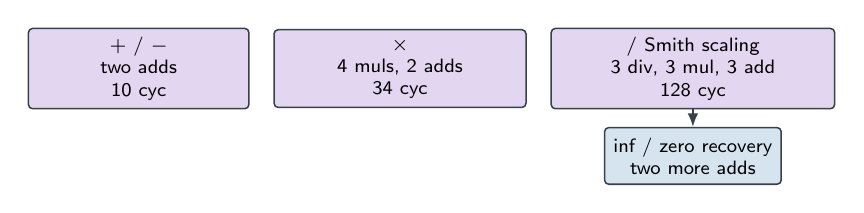
\begin{tikzpicture}[node distance=2.2mm and 3mm]
  \node[acc, minimum width=28mm] (add) {$+$ / $-$\\two adds\\10 cyc};
  \node[acc, right=of add, minimum width=32mm] (mul) {$\times$\\4 muls, 2 adds\\34 cyc};
  \node[acc, right=of mul, minimum width=36mm] (div) {$/$ Smith scaling\\3 div, 3 mul, 3 add\\128 cyc};
  \node[ctl, below=of div] (rec) {inf / zero recovery\\two more adds};
  \draw[arr] (div) -- (rec);
\end{tikzpicture}
\caption{Complex sequences, all on the scalar datapaths.
A complex value is two binary64 lanes.
Addition and subtraction are two adds.
Multiplication is CPython's four-multiply product.
Division is Smith's algorithm.
When that algorithm would return \texttt{nan+nanj} and exactly one operand holds an infinity, two further adds rebuild the result from signs.
Finite operands skip that recovery and keep the 128-cycle path.
A negative base raised to a fractional real power is not a complex result here; it traps \texttt{FPU\_EXCEPTION}.}
\label{fig:cplx}
\end{figure}


\subsection{Strings}

% String accelerator. Requires tikz_styles.tex.
\begin{figure}[htbp]
\centering
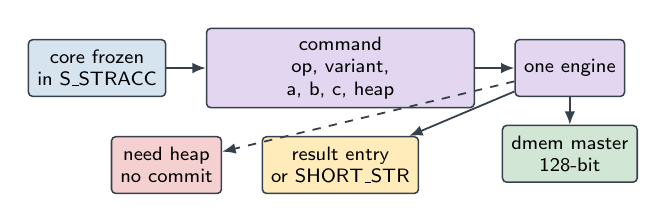
\begin{tikzpicture}[node distance=3.5mm and 5mm]
  \node[ctl] (core) {core frozen\\in S\_STRACC};
  \node[acc, right=of core, minimum width=34mm] (cmd)
    {command\\op, variant,\\a, b, c, heap};
  \node[acc, right=of cmd] (eng) {one engine};
  \node[mem, below=of eng] (dmem) {dmem master\\128-bit};
  \node[rf, below=of cmd] (res) {result entry\\or SHORT\_STR};
  \node[trap, left=of res] (oom) {need heap\\no commit};
  \draw[arr] (core) -- (cmd);
  \draw[arr] (cmd) -- (eng);
  \draw[arr] (eng) -- (dmem);
  \draw[arr] (eng) -- (res);
  \draw[darr] (eng) -- (oom);
\end{tikzpicture}
\caption{String accelerator (\texttt{pycore\_str\_accel}) as a master.
It runs only while the core is in \texttt{S\_STRACC}, so it cannot race L1D.
The command carries up to three tagged operands and the current heap pointer.
A result that fits in a \texttt{SHORT\_STR} is assembled in the destination register and does not allocate.
A result that needs a heap object either advances the bump pointer or returns \texttt{res\_need\_heap} with the heap untouched, so the core can collect and re-dispatch.
Small kind-1 concatenations whose result is at most 15 bytes never leave the execute fabric.}
\label{fig:stracc-top}
\end{figure}

\begin{figure}[htbp]
\centering
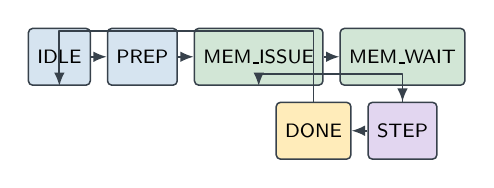
\begin{tikzpicture}[node distance=2mm and 2mm]
  \node[ctl] (idle) {IDLE};
  \node[ctl, right=of idle] (prep) {PREP};
  \node[mem, right=of prep] (iss) {MEM\_ISSUE};
  \node[mem, right=of iss] (wait) {MEM\_WAIT};
  \node[acc, below=of wait] (step) {STEP};
  \node[rf, left=of step] (done) {DONE};
  \draw[arr] (idle) -- (prep);
  \draw[arr] (prep) -- (iss);
  \draw[arr] (iss) -- (wait);
  \draw[arr] (wait) -- (step);
  \draw[arr] (step.west) -- (done.east);
  \draw[arr] (step.north) -- ++(0,0.35) -| (iss.south);
  \draw[arr] (done.north) -- ++(0,0.9) -| (idle.south);
\end{tikzpicture}
\caption{STRACC control.
\texttt{PREP} resolves a fast path (identity, empty operands, a case-map that the handle flags already answer) or selects an engine.
The memory loop issues one 128-bit beat, waits for \texttt{ack}, then steps the engine.
Kind~1, 2, and 4 move 16, 8, and 4 code units per beat.
Engines are copy, compare, search, hash, character, replace, join, trim, classify, map, affix, expand, and split.}
\label{fig:stracc-fsm}
\end{figure}

\begin{figure}[htbp]
\centering
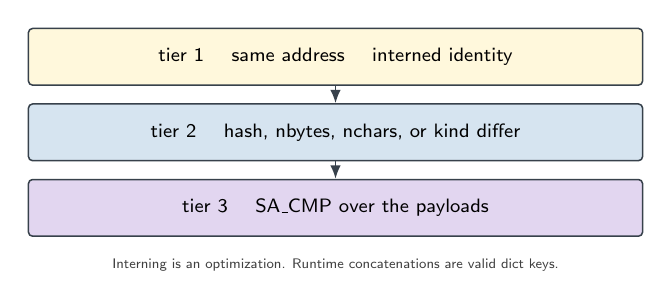
\begin{tikzpicture}[node distance=2.2mm]
  \node[hi, minimum width=78mm] (t1) {tier 1 \quad same address \quad interned identity};
  \node[ctl, minimum width=78mm, below=of t1] (t2)
    {tier 2 \quad hash, nbytes, nchars, or kind differ};
  \node[acc, minimum width=78mm, below=of t2] (t3)
    {tier 3 \quad SA\_CMP over the payloads};
  \foreach \p/\q in {t1/t2,t2/t3} \draw[arr] (\p) -- (\q);
  \node[anno, anchor=north] at ($(t3.south)+(0,-0.15)$)
    {Interning is an optimization. Runtime concatenations are valid dict keys.};
\end{tikzpicture}
\caption{String equality, cheapest test first.
Mixed \texttt{SHORT\_STR} and \texttt{LONG\_STR} compare unequal, because the canonical form says they cannot be the same text.
Same-tag long strings with matching metadata issue \texttt{SA\_CMP}, including ordering, not only \texttt{==}.
Dict and set probes take tier~3 when the metadata matches.
The hash in the handle is FNV-1a over the payload.}
\label{fig:streq}
\end{figure}

\begin{figure}[htbp]
\centering
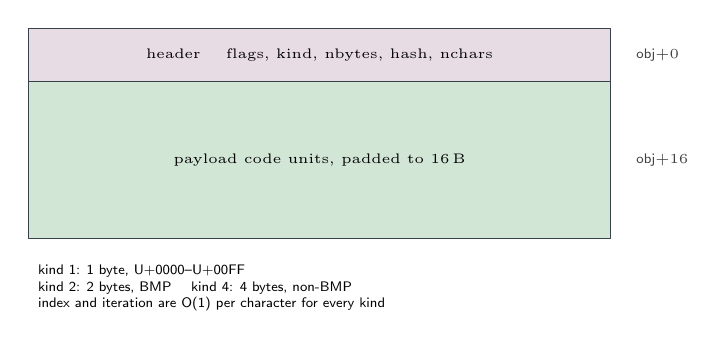
\begin{tikzpicture}[x=1cm,y=0.62cm]
  \fill[pyink] (0,3.2) rectangle (7.4,4.3);
  \fill[pymem] (0,0) rectangle (7.4,3.2);
  \draw[pyedge] (0,0) rectangle (7.4,4.3);
  \draw[pyedge] (0,3.2) -- (7.4,3.2);
  \node[font=\tiny] at (3.7,3.75) {header \quad flags, kind, nbytes, hash, nchars};
  \node[font=\tiny] at (3.7,1.6) {payload code units, padded to 16\,B};
  \node[anno, anchor=west] at (7.6,3.75) {obj$+0$};
  \node[anno, anchor=west] at (7.6,1.6) {obj$+16$};
  \node[font=\tiny\sffamily, align=left, anchor=north west] at (0,-0.35)
    {kind 1: 1 byte, U+0000--U+00FF\\
     kind 2: 2 bytes, BMP \quad kind 4: 4 bytes, non-BMP\\
     index and iteration are O(1) per character for every kind};
\end{tikzpicture}
\caption{Long-string object in the heap.
The header mirrors the handle, with the address field replaced by zero.
Payload bytes are fixed-width code units, as in CPython's \texttt{PyUnicodeObject}, not UTF-8.
Case mapping and the \texttt{is*} classifiers are a Latin-1 lookup table in the map and classify lanes.
A code point above U+00FF raises a recoverable firmware trap.
That is a performance boundary: the operation is still defined, it is just not done in the accelerator.
Structural operations (length, index, slice, compare, search, hash, split, trim, pad, \texttt{ord}) are exact for all of Unicode.}
\label{fig:strobj}
\end{figure}


\begin{table}[htbp]
\centering
\caption{STRACC commands (\texttt{PY\_SA\_*}).
The variant field selects a direction, a character class, or a case map.}
\label{tab:sa}
\small
\begin{tabular}{@{}clp{0.55\textwidth}@{}}
\toprule
Id & Command & Use \\
\midrule
0 & \texttt{CONCAT} & Long concatenation. Short results stay on the ALU. \\
1 & \texttt{REPEAT} & String repeat. \\
2 & \texttt{SLICE} & Slice of a long string. \\
3 & \texttt{PAD} & Left, right, or both. \\
4 & \texttt{CMP} & Payload compare after the handle rejects fail. \\
5 & \texttt{SEARCH} & Find, count, contains, prefix, suffix. \\
6 & \texttt{HASH} & FNV-1a into the handle. \\
7 & \texttt{CHAR\_AT} & O(1) index, every kind. \\
8 & \texttt{ITER\_NEXT} & One character per \texttt{FOR\_ITER} step. \\
9 & \texttt{REPLACE} & Substring replace. \\
10 & \texttt{JOIN} & Join over a list of strings. \\
11 & \texttt{TRIM} & Left, right, or both. \\
12 & \texttt{CLASSIFY} & Latin-1 \texttt{is*} tests. \\
13 & \texttt{MAP} & Latin-1 case map. \\
14 & \texttt{SPLIT} & Split, lines, partition. \\
15 & \texttt{AFFIX} & Prefix or suffix strip. \\
16 & \texttt{ZFILL} & Zero fill. \\
17 & \texttt{EXPANDTABS} & Tab expansion. \\
18 & \texttt{ORD} & One long character to an integer. \\
19 & \texttt{CHR} & Integer code point to one character. \\
\bottomrule
\end{tabular}
\end{table}

\subsection{Garbage collection}

% Garbage collector. Requires tikz_styles.tex.
\begin{figure}[htbp]
\centering
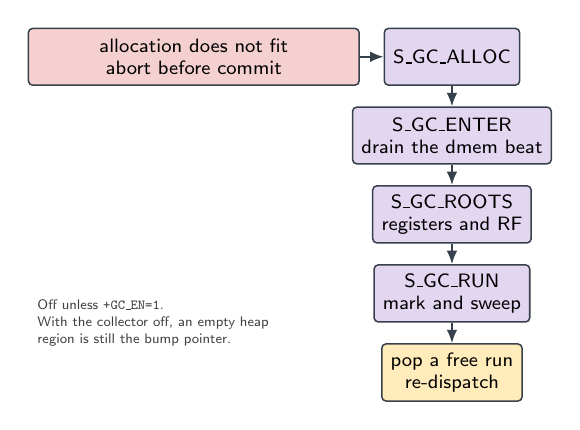
\begin{tikzpicture}[node distance=2.6mm and 3mm]
  \node[trap, minimum width=42mm] (fail) {allocation does not fit\\abort before commit};
  \node[acc, right=of fail] (alloc) {S\_GC\_ALLOC};
  \node[acc, below=of alloc] (enter) {S\_GC\_ENTER\\drain the dmem beat};
  \node[acc, below=of enter] (roots) {S\_GC\_ROOTS\\registers and RF};
  \node[acc, below=of roots] (run) {S\_GC\_RUN\\mark and sweep};
  \node[rf, below=of run] (resume) {pop a free run\\re-dispatch};
  \draw[arr] (fail) -- (alloc);
  \draw[arr] (alloc) -- (enter);
  \draw[arr] (enter) -- (roots);
  \draw[arr] (roots) -- (run);
  \draw[arr] (run) -- (resume);
  \node[anno, align=left, anchor=north west] at ($(fail.south west)+(0,-2.6)$)
    {Off unless \texttt{+GC\_EN=1}.\\
     With the collector off, an empty heap\\
     region is still the bump pointer.};
\end{tikzpicture}
\caption{Where a collection sits in the core.
Collections start at instruction boundaries.
An allocation that does not fit aborts that instruction before the first architectural commit, the core collects, and the instruction is fetched again.
\texttt{S\_GC\_ENTER} waits until any outstanding data beat from the abort has acknowledged, so a skip-clear cannot treat that read data as the first word of the static prune map.
If the free-run list still has a run, \texttt{S\_GC\_ALLOC} satisfies the request without a collection.}
\label{fig:gc-core}
\end{figure}

\begin{figure}[p]
\centering
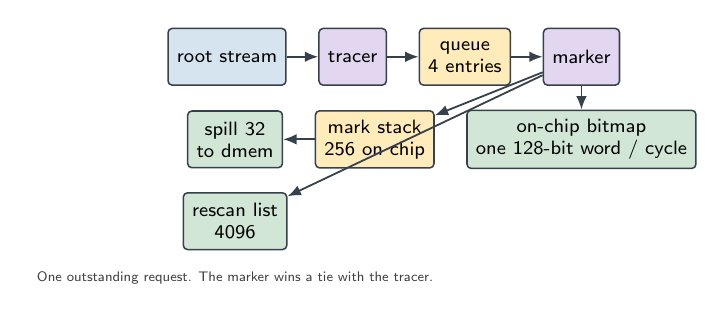
\begin{tikzpicture}[node distance=3mm and 4mm]
  \node[ctl] (roots) {root stream};
  \node[acc, right=of roots] (tr) {tracer};
  \node[rf, right=of tr] (q) {queue\\4 entries};
  \node[acc, right=of q] (mk) {marker};
  \node[mem, below=of mk] (bm) {on-chip bitmap\\one 128-bit word / cycle};
  \node[rf, left=of bm] (stk) {mark stack\\256 on chip};
  \node[mem, left=of stk] (spill) {spill 32\\to dmem};
  \node[mem, below=of spill] (re) {rescan list\\4096};
  \draw[arr] (roots) -- (tr);
  \draw[arr] (tr) -- (q);
  \draw[arr] (q) -- (mk);
  \draw[arr] (mk) -- (bm);
  \draw[arr] (mk) -- (stk);
  \draw[arr] (stk) -- (spill);
  \draw[arr] (mk) -- (re);
  \node[anno, align=left, anchor=north] at ($(re.south)+(0,-0.15)$)
    {One outstanding request. The marker wins a tie with the tracer.};
\end{tikzpicture}
\caption{Mark engine inside \texttt{pycore\_gc}.
The tracer walks memory-resident roots and the slots of each popped object, and emits child handles into the queue.
The marker tests the first granule of an extent, sets every granule, and pushes kinds that have children.
The bitmap is the on-chip array \texttt{bm\_q} (\texttt{PYCORE\_GC\_BITMAP\_WORDS} words, one bit per 16-byte granule).
The 256-entry on-chip stack spills its oldest 32 entries to \texttt{0xFC0000} when full and refills 32 when empty.
A pop scans at most 128 slots; the rest of the range is pushed first as a continuation, so a wide container holds at most 129 stack entries.
A child that still does not fit is left unmarked and the range is written once to the rescan list.
When the stack drains, that range is scanned again.
The collection is abandoned only when the rescan list itself is full.}
\label{fig:gc-mark}
\end{figure}

\begin{figure}[htbp]
\centering
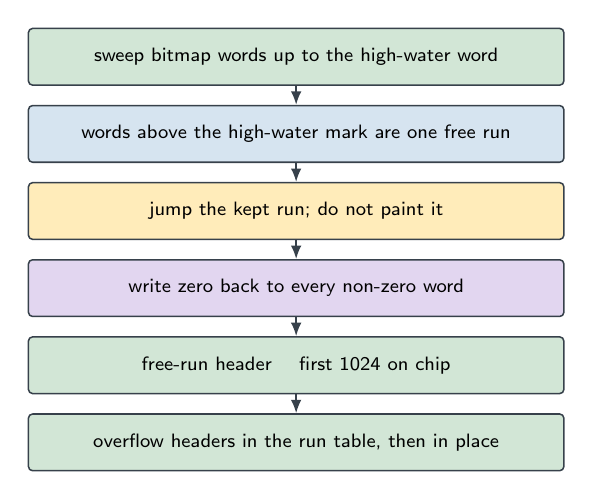
\begin{tikzpicture}[node distance=2.4mm]
  \node[mem, minimum width=68mm] (sw) {sweep bitmap words up to the high-water word};
  \node[ctl, minimum width=68mm, below=of sw] (skip) {words above the high-water mark are one free run};
  \node[rf, minimum width=68mm, below=of skip] (keep) {jump the kept run; do not paint it};
  \node[acc, minimum width=68mm, below=of keep] (clr) {write zero back to every non-zero word};
  \node[mem, minimum width=68mm, below=of clr] (hdr) {free-run header \quad first 1024 on chip};
  \node[mem, minimum width=68mm, below=of hdr] (ov) {overflow headers in the run table, then in place};
  \foreach \p/\q in {sw/skip,skip/keep,keep/clr,clr/hdr,hdr/ov} \draw[arr] (\p) -- (\q);
\end{tikzpicture}
\caption{Sweep and the free-run list.
The sweep clears the bitmap as it scans, so the next collection starts from a clean map.
After reset, and after an abandoned collection, the idle engine clears the bitmap in the background, one word per cycle.
Free runs are not a moving collector: a live object stays at its address.
The first 1024 run headers stay on chip.
Further headers go to \texttt{PYCORE\_GC\_RUN\_TABLE}.
Past that table they occupy the run's first granule, so the list has no fixed cap.
Allocator traffic in \texttt{S\_GC\_ALLOC} reads a header and zero-fills the granted line.}
\label{fig:gc-sweep}
\end{figure}

\begin{figure}[htbp]
\centering
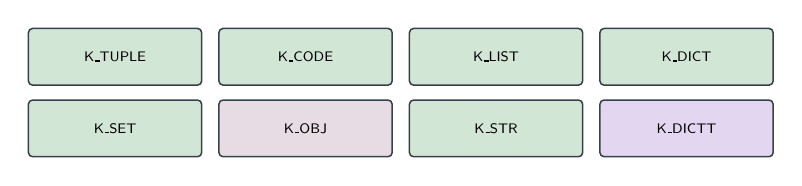
\begin{tikzpicture}[node distance=1.7mm and 2mm]
  \node[mem, font=\tiny\sffamily, minimum width=22mm] (k0) {K\_TUPLE};
  \node[mem, font=\tiny\sffamily, minimum width=22mm, right=of k0] (k1) {K\_CODE};
  \node[mem, font=\tiny\sffamily, minimum width=22mm, right=of k1] (k2) {K\_LIST};
  \node[mem, font=\tiny\sffamily, minimum width=22mm, right=of k2] (k3) {K\_DICT};
  \node[mem, font=\tiny\sffamily, minimum width=22mm, below=of k0] (k4) {K\_SET};
  \node[ink, font=\tiny\sffamily, minimum width=22mm, right=of k4] (k5) {K\_OBJ};
  \node[mem, font=\tiny\sffamily, minimum width=22mm, right=of k5] (k6) {K\_STR};
  \node[acc, font=\tiny\sffamily, minimum width=22mm, right=of k6] (k7) {K\_DICTT};
\end{tikzpicture}
\caption{Mark-stack entry kinds.
An entry is 67 bits: kind, size, and address.
\texttt{K\_TUPLE} is also the continuation kind for 32-byte slots (tuples, list buffers, set tables, dict order).
\texttt{K\_DICTT} continues a dict hash table, whose slots are 64 bytes.
\texttt{K\_OBJ} covers the \texttt{OBJECT} header kinds: instance, type, bound method, builtin, bytearray, exception, cell, and function.
Strings are traced for the object header; the payload bytes hold no pointers.}
\label{fig:gc-kinds}
\end{figure}


The collector is precise: it traces from tags, not from a conservative scan
of every word.
It does not move objects, so a handle cached in the ring or in a CODC payload
stays valid across a collection.
Roots are the live ring suffix, the frame descriptors, the exception stack,
the spill LIFO, the boot record, and the extra roots the image records for
builtins that the static prune map would otherwise hide.

\section{Containers, calls, and traps}
\label{sec:obj}

The container FSM is the accelerator for everything whose payload is a
pointer graph rather than a scalar.
Figure~\ref{fig:layouts} is the memory image those phases walk.
Figure~\ref{fig:split} is the cut between what the hart finishes and what
it hands to excore.

% Containers, objects, calls, and traps. Requires tikz_styles.tex.
\begin{figure}[p]
\centering
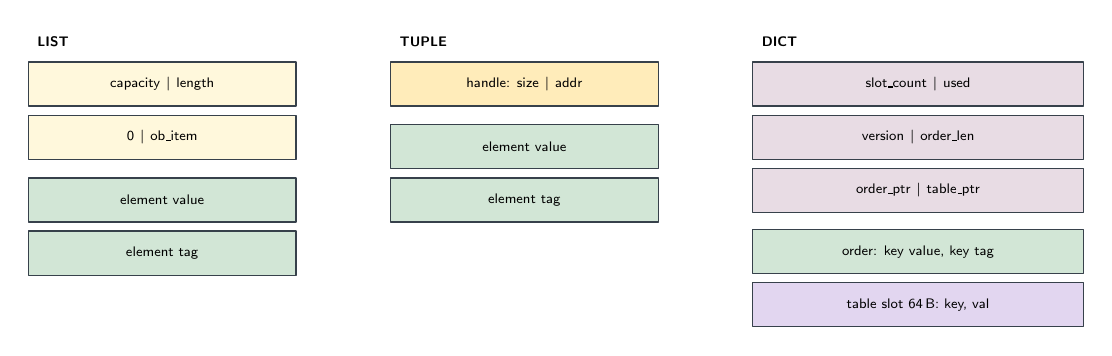
\begin{tikzpicture}[node distance=1.5mm and 3.5mm]
  % LIST
  \node[font=\tiny\sffamily\bfseries, anchor=west] at (0,0) {LIST};
  \node[slot, fill=pyhi, minimum width=34mm, anchor=north west] (lh) at (0,-0.25)
    {capacity $|$ length};
  \node[slot, fill=pyhi, minimum width=34mm, below=1mm of lh] (lb)
    {0 $|$ ob\_item};
  \node[slot, fill=pymem, minimum width=34mm, below=2.2mm of lb] (lv)
    {element value};
  \node[slot, fill=pymem, minimum width=34mm, below=1mm of lv] (lt)
    {element tag};
  % TUPLE
  \node[font=\tiny\sffamily\bfseries, anchor=west] at (4.6,0) {TUPLE};
  \node[slot, fill=pyrf, minimum width=34mm, anchor=north west] (th) at (4.6,-0.25)
    {handle: size $|$ addr};
  \node[slot, fill=pymem, minimum width=34mm, below=2.2mm of th] (tv)
    {element value};
  \node[slot, fill=pymem, minimum width=34mm, below=1mm of tv] (tt)
    {element tag};
  % DICT
  \node[font=\tiny\sffamily\bfseries, anchor=west] at (9.2,0) {DICT};
  \node[slot, fill=pyink, minimum width=42mm, anchor=north west] (dh) at (9.2,-0.25)
    {slot\_count $|$ used};
  \node[slot, fill=pyink, minimum width=42mm, below=1mm of dh] (dv)
    {version $|$ order\_len};
  \node[slot, fill=pyink, minimum width=42mm, below=1mm of dv] (dp)
    {order\_ptr $|$ table\_ptr};
  \node[slot, fill=pymem, minimum width=42mm, below=2mm of dp] (do)
    {order: key value, key tag};
  \node[slot, fill=pyacc, minimum width=42mm, below=1mm of do] (dt)
    {table slot 64\,B: key, val};
\end{tikzpicture}
\caption{Sequence and dict layout, 16-byte slots.
A list is a stable 32-byte object plus a relocatable element buffer.
Growing the buffer does not move the handle.
Each element is a value slot and a tag slot (32 bytes).
An empty list allocates no buffer.
A tuple stores its length in the handle, so it has no header.
A dict is a stable 48-byte object, an insertion-order key sidecar, and a relocatable open-addressed table.
Empty and deleted table slots are \texttt{UNINIT} and \texttt{TOMBSTONE}.
New keys append to the sidecar and bump \texttt{version}; a value overwrite does neither.
Iteration of a dict follows the sidecar, never hash-slot order.}
\label{fig:layouts}
\end{figure}

\begin{figure}[htbp]
\centering
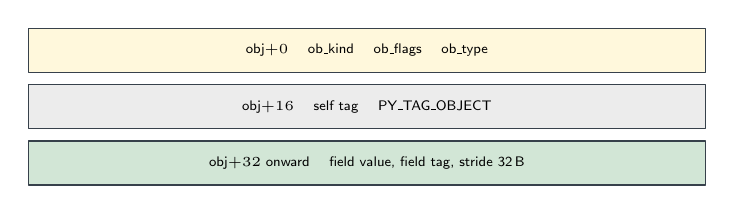
\begin{tikzpicture}[node distance=1.4mm]
  \node[slot, fill=pyhi, minimum width=86mm] (h)
    {obj$+0$ \quad ob\_kind \quad ob\_flags \quad ob\_type};
  \node[slot, fill=pyres, minimum width=86mm, below=of h] (t)
    {obj$+16$ \quad self tag \quad PY\_TAG\_OBJECT};
  \node[slot, fill=pymem, minimum width=86mm, below=of t] (f)
    {obj$+32$ onward \quad field value, field tag, stride 32\,B};
\end{tikzpicture}
\caption{General heap object.
The handle is \texttt{OBJECT} plus the object address.
The kind is not in the tag: \texttt{LOAD\_ATTR} and \texttt{CALL} read \texttt{ob\_head} first.
Kinds in use are instance (dict at field 0), type (dict, base, name), bound method, builtin, exception, cell, and function (code object plus a cell tuple).
Lists, dicts, and sets are \texttt{MUT\_COLLEC}, not \texttt{OBJECT}.
Strings are \texttt{SHORT\_STR} or \texttt{LONG\_STR}.
Range has its own tag.}
\label{fig:object}
\end{figure}

\begin{figure}[htbp]
\centering
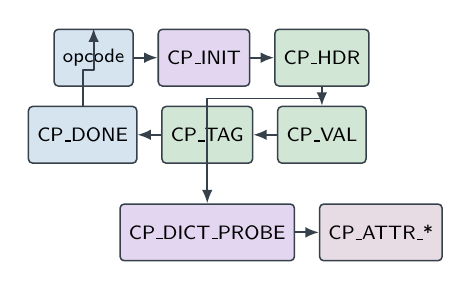
\begin{tikzpicture}[node distance=2.4mm and 3mm]
  \node[ctl] (op) {opcode};
  \node[acc, right=of op] (init) {CP\_INIT};
  \node[mem, right=of init] (hdr) {CP\_HDR};
  \node[mem, below=of hdr] (val) {CP\_VAL};
  \node[mem, left=of val] (tag) {CP\_TAG};
  \node[ctl, left=of tag] (done) {CP\_DONE};
  \node[acc, below=5mm of tag] (probe) {CP\_DICT\_PROBE};
  \node[ink, right=of probe] (attr) {CP\_ATTR\_*};
  \draw[arr] (op) -- (init);
  \draw[arr] (init) -- (hdr);
  \draw[arr] (hdr) -- (val);
  \draw[arr] (val) -- (tag);
  \draw[arr] (tag) -- (done);
  \draw[arr] (hdr.south) -- ++(0,-0.15) -| (probe.north);
  \draw[arr] (probe) -- (attr);
  \draw[arr] (done.north) -- ++(0,0.45) -| (op.north);
\end{tikzpicture}
\caption{Container microcode (\texttt{S\_CONTAINER}).
Decode sets \texttt{dec\_is\_container} and execute transfers here, skipping \texttt{S\_MEM} and \texttt{S\_WB}.
The phase register is \texttt{container\_phase\_r}.
Shared phases read or write a header, a value slot, and a tag slot, then \texttt{CP\_DONE} returns to fetch.
Dict and set operations insert a probe loop.
Attribute operations insert a walk of the instance dict and the type MRO.
The arms live in the \texttt{pycore\_cont\_*.svh} files included into the core.
Fifty-six of the sixty-four \texttt{CONT\_*} codes are in use.
A recoverable failure sets \texttt{trap\_marshal\_pending\_r} and \texttt{CP\_DONE} leaves for the mailbox instead of fetch.}
\label{fig:contfsm}
\end{figure}

\begin{figure}[p]
\centering
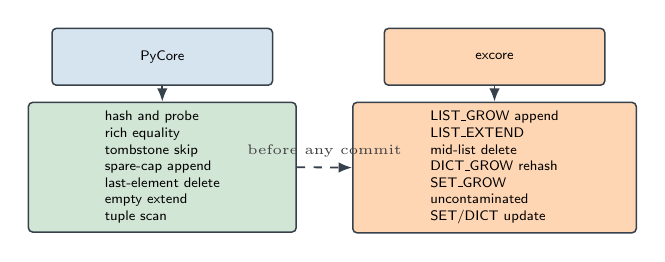
\begin{tikzpicture}[node distance=2mm and 2.4mm]
  \node[ctl, minimum width=28mm, font=\tiny\sffamily] (py) {PyCore};
  \node[ex, minimum width=28mm, font=\tiny\sffamily, right=14mm of py] (ex) {excore};
  \node[mem, font=\tiny\sffamily, below=of py, minimum width=34mm, align=left] (pyl)
    {hash and probe\\rich equality\\tombstone skip\\spare-cap append\\last-element delete\\empty extend\\tuple scan};
  \node[ex, font=\tiny\sffamily, below=of ex, minimum width=36mm, align=left] (exl)
    {LIST\_GROW append\\LIST\_EXTEND\\mid-list delete\\DICT\_GROW rehash\\SET\_GROW\\uncontaminated\\SET/DICT update};
  \draw[arr] (py) -- (pyl);
  \draw[arr] (ex) -- (exl);
  \draw[darr] (pyl.east) -- node[anno, above, font=\tiny] {before any commit} (exl.west);
\end{tikzpicture}
\caption{What stays on PyCore, and what is finished by excore.
Hashing, equality, and the open-addressed probe stay on the hart.
Capacity changes and the long memmoves go to firmware, which must complete the semantic effect rather than resize and retry.
The trap is raised before any register-file, heap, or data-memory commit, which is what makes a later \texttt{RETRY} legal.
No current handler returns \texttt{RETRY}; they return \texttt{COMPLETED}.
Contaminated containers (an \texttt{OBJECT} key or element) and tuple-sourced set updates stay on PyCore in \texttt{pycore\_cont\_bulk}.}
\label{fig:split}
\end{figure}

\begin{figure}[htbp]
\centering
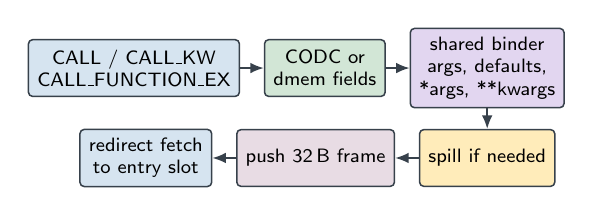
\begin{tikzpicture}[node distance=2.6mm and 3mm]
  \node[ctl] (call) {CALL / CALL\_KW\\CALL\_FUNCTION\_EX};
  \node[mem, right=of call] (codc) {CODC or\\dmem fields};
  \node[acc, right=of codc] (bind) {shared binder\\args, defaults,\\*args, **kwargs};
  \node[rf, below=of bind] (spill) {spill if needed};
  \node[ink, left=of spill] (frame) {push 32\,B frame};
  \node[ctl, left=of frame] (go) {redirect fetch\\to entry slot};
  \draw[arr] (call) -- (codc);
  \draw[arr] (codc) -- (bind);
  \draw[arr] (bind) -- (spill);
  \draw[arr] (spill) -- (frame);
  \draw[arr] (frame) -- (go);
\end{tikzpicture}
\caption{Call, as it sits among the other machines.
The phase-by-phase binder is the sibling note \texttt{call\_fsm.tex}.
A user function is a code object, except a closure, which is an \texttt{OBK\_FUNCTION} wrapping the code object and a cell tuple.
\texttt{CALL} checks the callable, binds positional and keyword arguments against \texttt{co\_varnames}, then enters the frame manager.
Builtins with a hardware fast path (\texttt{len}, \texttt{range}, \texttt{set}, two-argument \texttt{max}, \texttt{int} and \texttt{str} conversion) dispatch inside this FSM.
Other builtin calls raise the recoverable \texttt{PY\_TRAP\_BUILTIN\_CALL}.
Return pops the descriptor, writes the result into the caller's ring, and fills any spilled prefix the caller needs.}
\label{fig:call}
\end{figure}

\begin{figure}[htbp]
\centering
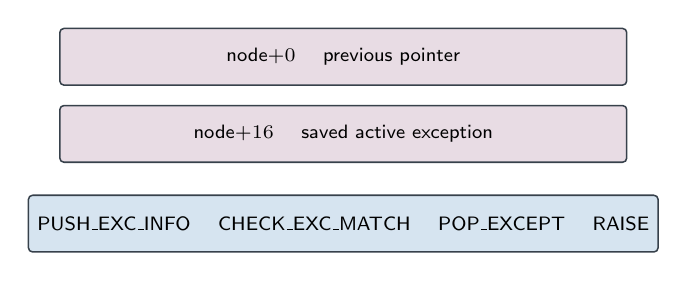
\begin{tikzpicture}[node distance=2.4mm]
  \node[ink, minimum width=72mm] (n0)
    {node$+0$ \quad previous pointer};
  \node[ink, minimum width=72mm, below=of n0] (n1)
    {node$+16$ \quad saved active exception};
  \node[ctl, below=4mm of n1] (ops)
    {PUSH\_EXC\_INFO \quad CHECK\_EXC\_MATCH \quad POP\_EXCEPT \quad RAISE};
\end{tikzpicture}
\caption{Exception-info stack.
The arena is 4\,KB at \texttt{0xF00000}, 32 bytes per node, depth 128.
It is a data-memory LIFO owned by \texttt{pycore\_exc\_stack}, separate from both the operand ring and the call-frame stack.
The native-method table and the \texttt{StopIteration} sidecar sit in the same arena.
\texttt{FOR\_ITER} exhaustion compares the raised type by identity with the sidecar latched at boot, and redirects to \texttt{POP\_ITER} without a user handler.
A user \texttt{raise} with no handler is still fatal \texttt{PY\_TRAP\_RAISE}.}
\label{fig:exc}
\end{figure}

\begin{figure}[htbp]
\centering
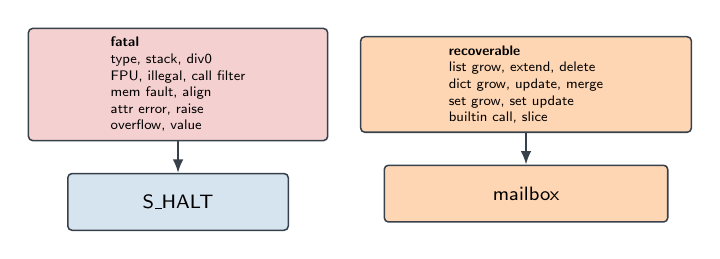
\begin{tikzpicture}[node distance=2.2mm and 4mm]
  \node[trap, minimum width=38mm, align=left, font=\tiny\sffamily] (fat)
    {\textbf{fatal}\\
     type, stack, div0\\
     FPU, illegal, call filter\\
     mem fault, align\\
     attr error, raise\\
     overflow, value};
  \node[ex, minimum width=42mm, align=left, font=\tiny\sffamily, right=of fat] (rec)
    {\textbf{recoverable}\\
     list grow, extend, delete\\
     dict grow, update, merge\\
     set grow, set update\\
     builtin call, slice};
  \node[ctl, minimum width=28mm, below=4mm of fat] (halt) {S\_HALT};
  \node[ex, minimum width=36mm, below=4mm of rec] (mb) {mailbox};
  \draw[arr] (fat) -- (halt);
  \draw[arr] (rec) -- (mb);
\end{tikzpicture}
\caption{Trap classes.
\texttt{pycore\_trap\_recoverable} in \texttt{pycore\_defs.svh} is the split.
With excore disabled, a recoverable code is fatal too.
\texttt{COMPLETED} applies the popped and pushed entries and resumes at the next instruction.
\texttt{RETRY} redirects fetch to the same PC.
\texttt{FATAL} enters \texttt{pycore\_trap} with the firmware's code.
\texttt{NEED\_HEAP} collects if the collector is enabled, and halts otherwise.}
\label{fig:traps}
\end{figure}

\begin{figure}[htbp]
\centering
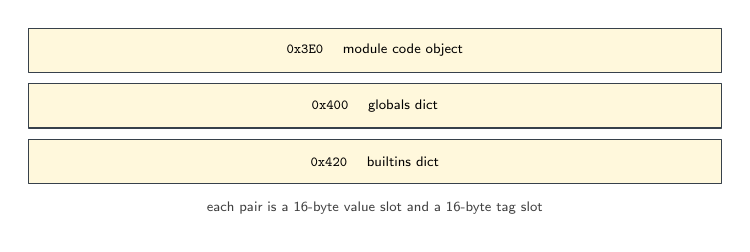
\begin{tikzpicture}[node distance=1.3mm]
  \node[slot, fill=pyhi, minimum width=88mm] (b0) {\texttt{0x3E0} \quad module code object};
  \node[slot, fill=pyhi, minimum width=88mm, below=of b0] (b1) {\texttt{0x400} \quad globals dict};
  \node[slot, fill=pyhi, minimum width=88mm, below=of b1] (b2) {\texttt{0x420} \quad builtins dict};
  \node[anno, below=1mm of b2] {each pair is a 16-byte value slot and a 16-byte tag slot};
\end{tikzpicture}
\caption{Boot record, read by \texttt{S\_BOOT} when \texttt{BOOT\_EN=1}.
The walker checks the tags, caches \texttt{co\_consts} and \texttt{co\_names}, latches the globals and builtins bases, and redirects fetch to the module entry slot.
A serialized code object is eight tagged fields: entry slot, consts, names, packed metadata, defaults, varnames, keyword defaults, and the raw exception table.
\texttt{LOAD\_CONST} indexes \texttt{co\_consts} with two data reads (value, then tag).
\texttt{LOAD\_GLOBAL} and \texttt{LOAD\_NAME} probe the frame globals and then the builtins dict; a miss is \texttt{MEM\_FAULT}.}
\label{fig:boot}
\end{figure}


\begin{table}[htbp]
\centering
\caption{Set layout, the compact cousin of the dict.
No order sidecar. Elements only. The same hash, rich equality, and tombstone rules.}
\label{tab:set}
\small
\begin{tabular}{@{}lp{0.68\textwidth}@{}}
\toprule
Address & Contents \\
\midrule
obj$+0$ & \texttt{slot\_count}, \texttt{used} \\
obj$+16$ & \texttt{table\_ptr} (0 when the table is empty) \\
table $+\,32i$ & element value, then element tag \\
\bottomrule
\end{tabular}
\end{table}

\texttt{BUILD\_SET} and \texttt{SET\_ADD} probe and insert on PyCore.
A load of two thirds or more raises \texttt{SET\_GROW}.
\texttt{DELETE\_SUBSCR} and \texttt{STORE\_SUBSCR} on a set are type errors.

\subsection{Iterator payload}

\texttt{GET\_ITER} rewrites a list, tuple, range, string, dict, or set into
an \texttt{ITER} value.
The 128-bit payload is
\[
  \mathrm{magic}[127{:}120],\;
  \mathrm{kind}[119{:}116],\;
  \mathrm{aux}[115{:}96],\;
  \mathrm{index}[95{:}64],\;
  \mathrm{size}[63{:}32],\;
  \mathrm{addr}[31{:}0].
\]
Kinds 0--3 are list, tuple, range, and string.
Kind 4 is a heap iterator for a user \texttt{\_\_iter\_\_}.
Kinds 5 and 6 are dict and set.
Dict and set iterators snapshot a mutation counter and raise
\texttt{PY\_TRAP\_TYPE} if the container changes size during the loop.

\section{Figure index for the paper}
\label{sec:index}

A first paper figure set, in the order a systems section usually wants them:

\begin{enumerate}
\item Figure~\ref{fig:twocore} --- the chip: two harts, one heap.
\item Figure~\ref{fig:hart} --- what is inside PyCore.
\item Figure~\ref{fig:entry} and Figure~\ref{fig:tags} --- the value the
      datapath actually carries.
\item Figure~\ref{fig:ring} and Figure~\ref{fig:spill} --- the register stack.
\item Figure~\ref{fig:hier} and Figure~\ref{fig:map} --- memory.
\item Figure~\ref{fig:accel-all} --- accelerators on one page.
\item Figure~\ref{fig:exec}, Figure~\ref{fig:fpu}, Figure~\ref{fig:stracc-top},
      Figure~\ref{fig:gc-mark} --- one diagram of how each family works.
\item Figure~\ref{fig:layouts} and Figure~\ref{fig:split} --- objects, and
      the cut with excore.
\end{enumerate}

The remaining figures are the working drawings underneath those: cache
microarchitecture, the data-port mux, each integer and floating-point
datapath, the string engines, the collector's sweep, the container phases,
boot, and the trap split.

\end{document}
